\begin{figure*}
    \centering
    \begin{subfigure}{0.45\linewidth}
        \centering
        \begin{adjustbox}{width=\textwidth}
            % This file was created by tikzplotlib v0.9.5.
\begin{tikzpicture}





\begin{axis}[
axis background/.style={fill=white!89.8039215686275!black},
axis line style={white},
legend cell align={left},
legend style={fill opacity=0.8, draw opacity=1, text opacity=1, at={(0.03,0.03)}, anchor=south west, draw=white!80!black, fill=white!89.8039215686275!black},
%log basis y={10},
tick align=outside,
tick pos=left,
title={MNIST training},
x grid style={white},
xlabel={time},
xmajorgrids,
xmin=-1.8444581, xmax=48.6648733,
xtick style={color=white!33.3333333333333!black},
y grid style={white},
ylabel={accuracy},
ymajorgrids,
ymin=23.6870160941979, ymax=107.098952012845,
%ymode=log,
ytick style={color=white!33.3333333333333!black}
]
\path [fill=cudnn, fill opacity=0.2, very thin]
(axis cs:0.4782266,70.409309)
--(axis cs:0.4782266,25.368546)
--(axis cs:0.9232159,52.610394)
--(axis cs:1.3681511,46.064877)
--(axis cs:1.813181,59.719769)
--(axis cs:2.2582623,72.457542)
--(axis cs:2.7032656,79.869225)
--(axis cs:3.1482741,86.851219)
--(axis cs:3.5932938,91.06488)
--(axis cs:4.038329,84.553329)
--(axis cs:4.4834467,93.05027)
--(axis cs:4.9285291,95.606316)
--(axis cs:5.3737088,95.278534)
--(axis cs:5.8189509,96.363792)
--(axis cs:6.2641013,96.418137)
--(axis cs:6.7093389,96.908966)
--(axis cs:7.1544196,77.438858)
--(axis cs:7.5995075,92.370926)
--(axis cs:8.0445662,94.998299)
--(axis cs:8.489797,96.7714)
--(axis cs:8.9349618,97.246941)
--(axis cs:9.3799734,97.257133)
--(axis cs:9.8251089,97.623978)
--(axis cs:10.2701673,97.712296)
--(axis cs:10.7152981,97.73098)
--(axis cs:11.1603761,97.7089)
--(axis cs:11.6055043,97.715691)
--(axis cs:12.0506865,97.829483)
--(axis cs:12.4958184,97.832878)
--(axis cs:12.9409165,96.295853)
--(axis cs:13.3859977,97.927986)
--(axis cs:13.8311519,97.729279)
--(axis cs:14.2761924,98.254074)
--(axis cs:14.7213617,97.005775)
--(axis cs:15.1664679,98.388245)
--(axis cs:15.6114732,98.25238)
--(axis cs:16.0566084,98.410324)
--(axis cs:16.501812,98.552986)
--(axis cs:16.9470843,98.328804)
--(axis cs:17.3922826,98.226906)
--(axis cs:17.8373712,97.515282)
--(axis cs:18.282443,98.357674)
--(axis cs:18.7275257,98.49015)
--(axis cs:19.1725744,98.372963)
--(axis cs:19.6176348,98.576767)
--(axis cs:20.0626668,98.637909)
--(axis cs:20.5078902,98.340691)
--(axis cs:20.9531108,98.422218)
--(axis cs:21.398351,98.510529)
--(axis cs:21.843595,98.739807)
--(axis cs:22.2887302,98.524117)
--(axis cs:22.7337989,98.707542)
--(axis cs:23.1789517,98.603943)
--(axis cs:23.6240882,98.758492)
--(axis cs:24.0692921,98.683762)
--(axis cs:24.5144183,98.773781)
--(axis cs:24.9595631,96.908966)
--(axis cs:25.4046424,98.656593)
--(axis cs:25.8497148,97.922897)
--(axis cs:26.2947474,98.629417)
--(axis cs:26.7398837,98.894363)
--(axis cs:27.1848716,98.77887)
--(axis cs:27.6299501,98.751701)
--(axis cs:28.0749458,98.945312)
--(axis cs:28.5199763,97.365829)
--(axis cs:28.9651299,96.110733)
--(axis cs:29.4101996,98.704147)
--(axis cs:29.8552906,98.901154)
--(axis cs:30.3002666,98.972488)
--(axis cs:30.7453382,99.031929)
--(axis cs:31.190327,97.476219)
--(axis cs:31.6354719,99.040421)
--(axis cs:32.0805844,98.158966)
--(axis cs:32.5257041,98.904549)
--(axis cs:32.9708542,99.011551)
--(axis cs:33.4160196,99.09137)
--(axis cs:33.8610718,99.217049)
--(axis cs:34.3061513,99.118546)
--(axis cs:34.7512437,89.349525)
--(axis cs:35.1961926,95.864471)
--(axis cs:35.6411077,98.028191)
--(axis cs:36.0860932,98.462975)
--(axis cs:36.5310712,98.615829)
--(axis cs:36.9761031,98.085938)
--(axis cs:37.4211117,98.965691)
--(axis cs:37.8660675,98.994568)
--(axis cs:38.3110037,99.011551)
--(axis cs:38.7560695,99.188179)
--(axis cs:39.2011195,99.077782)
--(axis cs:39.6460269,99.099861)
--(axis cs:40.0909067,99.284988)
--(axis cs:40.5359762,98.972488)
--(axis cs:40.9810362,99.191574)
--(axis cs:41.4260278,99.235733)
--(axis cs:41.8710576,99.135529)
--(axis cs:42.316014,99.179688)
--(axis cs:42.760984,94.772415)
--(axis cs:43.2059163,98.907951)
--(axis cs:43.6508853,99.094772)
--(axis cs:44.0959597,98.220108)
--(axis cs:44.5409831,99.150818)
--(axis cs:44.5409831,99.867531)
--(axis cs:44.5409831,99.867531)
--(axis cs:44.0959597,99.835258)
--(axis cs:43.6508853,99.852242)
--(axis cs:43.2059163,99.821671)
--(axis cs:42.760984,99.874321)
--(axis cs:42.316014,99.853943)
--(axis cs:41.8710576,99.83696)
--(axis cs:41.4260278,99.808083)
--(axis cs:40.9810362,99.806389)
--(axis cs:40.5359762,99.84375)
--(axis cs:40.0909067,99.819969)
--(axis cs:39.6460269,99.802986)
--(axis cs:39.2011195,99.816574)
--(axis cs:38.7560695,99.842049)
--(axis cs:38.3110037,99.804688)
--(axis cs:37.8660675,99.796196)
--(axis cs:37.4211117,99.813179)
--(axis cs:36.9761031,99.772415)
--(axis cs:36.5310712,99.758835)
--(axis cs:36.0860932,99.772415)
--(axis cs:35.6411077,99.845451)
--(axis cs:35.1961926,99.797897)
--(axis cs:34.7512437,99.729958)
--(axis cs:34.3061513,99.774117)
--(axis cs:33.8610718,99.808083)
--(axis cs:33.4160196,99.733353)
--(axis cs:32.9708542,99.750343)
--(axis cs:32.5257041,99.733353)
--(axis cs:32.0805844,99.721466)
--(axis cs:31.6354719,99.729958)
--(axis cs:31.190327,99.801292)
--(axis cs:30.7453382,99.772415)
--(axis cs:30.3002666,99.735054)
--(axis cs:29.8552906,99.711281)
--(axis cs:29.4101996,99.675613)
--(axis cs:28.9651299,99.712975)
--(axis cs:28.5199763,99.68071)
--(axis cs:28.0749458,99.636551)
--(axis cs:27.6299501,99.690895)
--(axis cs:27.1848716,99.651833)
--(axis cs:26.7398837,99.63485)
--(axis cs:26.2947474,99.638245)
--(axis cs:25.8497148,99.611076)
--(axis cs:25.4046424,99.622963)
--(axis cs:24.9595631,99.638245)
--(axis cs:24.5144183,99.575409)
--(axis cs:24.0692921,99.558426)
--(axis cs:23.6240882,99.522758)
--(axis cs:23.1789517,99.56012)
--(axis cs:22.7337989,99.590691)
--(axis cs:22.2887302,99.548233)
--(axis cs:21.843595,99.565216)
--(axis cs:21.398351,99.536346)
--(axis cs:20.9531108,99.527855)
--(axis cs:20.5078902,99.495583)
--(axis cs:20.0626668,99.446335)
--(axis cs:19.6176348,99.519363)
--(axis cs:19.1725744,99.444633)
--(axis cs:18.7275257,99.383492)
--(axis cs:18.282443,99.432747)
--(axis cs:17.8373712,99.386887)
--(axis cs:17.3922826,99.366508)
--(axis cs:16.9470843,99.352921)
--(axis cs:16.501812,99.393684)
--(axis cs:16.0566084,99.332542)
--(axis cs:15.6114732,99.369904)
--(axis cs:15.1664679,99.279892)
--(axis cs:14.7213617,99.249321)
--(axis cs:14.2761924,99.273094)
--(axis cs:13.8311519,99.240829)
--(axis cs:13.3859977,99.193275)
--(axis cs:12.9409165,99.099861)
--(axis cs:12.4958184,99.116844)
--(axis cs:12.0506865,99.084579)
--(axis cs:11.6055043,98.947014)
--(axis cs:11.1603761,98.953804)
--(axis cs:10.7152981,98.884171)
--(axis cs:10.2701673,98.87738)
--(axis cs:9.8251089,98.880775)
--(axis cs:9.3799734,98.792458)
--(axis cs:8.9349618,98.688858)
--(axis cs:8.489797,98.651497)
--(axis cs:8.0445662,98.649796)
--(axis cs:7.5995075,98.517326)
--(axis cs:7.1544196,98.423912)
--(axis cs:6.7093389,98.27446)
--(axis cs:6.2641013,98.125)
--(axis cs:5.8189509,97.972145)
--(axis cs:5.3737088,97.710594)
--(axis cs:4.9285291,97.522079)
--(axis cs:4.4834467,97.347145)
--(axis cs:4.038329,96.954826)
--(axis cs:3.5932938,97.209579)
--(axis cs:3.1482741,96.768005)
--(axis cs:2.7032656,96.051292)
--(axis cs:2.2582623,95.453468)
--(axis cs:1.813181,92.987434)
--(axis cs:1.3681511,88.580162)
--(axis cs:0.9232159,85.02887)
--(axis cs:0.4782266,70.409309)
--cycle;

\path [fill=libtorch, fill opacity=0.2, very thin]
(axis cs:0.4514206,90.555367)
--(axis cs:0.4514206,88.639603)
--(axis cs:0.9022784,97.686821)
--(axis cs:1.3534231,98.688858)
--(axis cs:1.8043956,99.120247)
--(axis cs:2.255545,99.400475)
--(axis cs:2.7067402,99.570312)
--(axis cs:3.1576851,99.588997)
--(axis cs:3.6087245,99.728264)
--(axis cs:4.0595726,99.818275)
--(axis cs:4.5104858,99.826767)
--(axis cs:4.9615293,99.894699)
--(axis cs:5.4125489,99.876022)
--(axis cs:5.863595,99.894699)
--(axis cs:6.314577,99.877716)
--(axis cs:6.7656383,99.840355)
--(axis cs:7.2164882,99.860733)
--(axis cs:7.6673026,99.867531)
--(axis cs:8.1183483,99.921875)
--(axis cs:8.5693941,99.903191)
--(axis cs:9.0203725,99.882812)
--(axis cs:9.4712526,99.916779)
--(axis cs:9.9224924,99.949051)
--(axis cs:10.3732561,99.94735)
--(axis cs:10.8243106,99.942253)
--(axis cs:11.2752643,99.964333)
--(axis cs:11.7258814,99.926971)
--(axis cs:12.1768194,99.949051)
--(axis cs:12.6278308,99.972824)
--(axis cs:13.0786394,99.957542)
--(axis cs:13.529549,99.943954)
--(axis cs:13.9803709,99.97113)
--(axis cs:14.4313935,99.974525)
--(axis cs:14.8823161,99.967728)
--(axis cs:15.3333867,99.983017)
--(axis cs:15.7843831,99.977921)
--(axis cs:16.2350727,99.950745)
--(axis cs:16.6861017,99.966034)
--(axis cs:17.1369704,99.954147)
--(axis cs:17.5877198,99.950745)
--(axis cs:18.0386275,99.967728)
--(axis cs:18.489467,99.969429)
--(axis cs:18.9403415,99.981316)
--(axis cs:19.3913184,99.974525)
--(axis cs:19.8423633,99.94735)
--(axis cs:20.2933696,99.972824)
--(axis cs:20.7443091,99.94735)
--(axis cs:21.1955409,99.904892)
--(axis cs:21.6463799,99.972824)
--(axis cs:22.0973493,99.976219)
--(axis cs:22.548191,99.981316)
--(axis cs:22.9990786,99.972824)
--(axis cs:23.4500047,99.977921)
--(axis cs:23.9008287,99.967728)
--(axis cs:24.3516837,99.913383)
--(axis cs:24.80285,99.976219)
--(axis cs:25.2538591,99.950745)
--(axis cs:25.7046932,99.972824)
--(axis cs:26.1559451,99.981316)
--(axis cs:26.6070184,99.979622)
--(axis cs:27.0579189,99.979622)
--(axis cs:27.5088431,99.986412)
--(axis cs:27.9599997,99.989807)
--(axis cs:28.4110492,99.996605)
--(axis cs:28.8618921,99.986412)
--(axis cs:29.3128527,99.986412)
--(axis cs:29.7638637,99.977921)
--(axis cs:30.2149583,99.991508)
--(axis cs:30.6660081,99.986412)
--(axis cs:31.1165665,99.979622)
--(axis cs:31.5673747,99.979622)
--(axis cs:32.0183621,99.974525)
--(axis cs:32.4694334,99.983017)
--(axis cs:32.9205166,99.97113)
--(axis cs:33.3712593,99.97113)
--(axis cs:33.8220931,99.974525)
--(axis cs:34.2729178,99.966034)
--(axis cs:34.7240035,99.984718)
--(axis cs:35.1753118,99.991508)
--(axis cs:35.626446,99.991508)
--(axis cs:36.0774815,99.988113)
--(axis cs:36.5283737,99.986412)
--(axis cs:36.9791905,99.959236)
--(axis cs:37.4303597,99.943954)
--(axis cs:37.881495,99.935463)
--(axis cs:38.3325126,99.923576)
--(axis cs:38.7835199,99.891304)
--(axis cs:39.234442,99.972824)
--(axis cs:39.6855538,99.938858)
--(axis cs:40.1366098,99.926971)
--(axis cs:40.5878227,99.928665)
--(axis cs:41.0389411,99.979622)
--(axis cs:41.4898508,99.983017)
--(axis cs:41.9410489,99.952446)
--(axis cs:42.392293,99.99321)
--(axis cs:42.8432532,99.994904)
--(axis cs:43.2942657,99.991508)
--(axis cs:43.7452244,99.99321)
--(axis cs:44.1960269,99.99321)
--(axis cs:44.6471278,99.996605)
--(axis cs:45.0979666,99.986412)
--(axis cs:45.0979666,100)
--(axis cs:45.0979666,100)
--(axis cs:44.6471278,100)
--(axis cs:44.1960269,100)
--(axis cs:43.7452244,100)
--(axis cs:43.2942657,100)
--(axis cs:42.8432532,100)
--(axis cs:42.392293,100)
--(axis cs:41.9410489,100)
--(axis cs:41.4898508,100)
--(axis cs:41.0389411,100)
--(axis cs:40.5878227,100)
--(axis cs:40.1366098,100)
--(axis cs:39.6855538,100)
--(axis cs:39.234442,100)
--(axis cs:38.7835199,100)
--(axis cs:38.3325126,100)
--(axis cs:37.881495,100)
--(axis cs:37.4303597,100)
--(axis cs:36.9791905,100)
--(axis cs:36.5283737,100)
--(axis cs:36.0774815,100)
--(axis cs:35.626446,100)
--(axis cs:35.1753118,100)
--(axis cs:34.7240035,100)
--(axis cs:34.2729178,100)
--(axis cs:33.8220931,100)
--(axis cs:33.3712593,100)
--(axis cs:32.9205166,100)
--(axis cs:32.4694334,100)
--(axis cs:32.0183621,100)
--(axis cs:31.5673747,100)
--(axis cs:31.1165665,100)
--(axis cs:30.6660081,100)
--(axis cs:30.2149583,100)
--(axis cs:29.7638637,100)
--(axis cs:29.3128527,100)
--(axis cs:28.8618921,100)
--(axis cs:28.4110492,100)
--(axis cs:27.9599997,100)
--(axis cs:27.5088431,100)
--(axis cs:27.0579189,100)
--(axis cs:26.6070184,100)
--(axis cs:26.1559451,100)
--(axis cs:25.7046932,100)
--(axis cs:25.2538591,100)
--(axis cs:24.80285,100)
--(axis cs:24.3516837,100)
--(axis cs:23.9008287,100)
--(axis cs:23.4500047,100)
--(axis cs:22.9990786,100)
--(axis cs:22.548191,100)
--(axis cs:22.0973493,100)
--(axis cs:21.6463799,100)
--(axis cs:21.1955409,100)
--(axis cs:20.7443091,100)
--(axis cs:20.2933696,100)
--(axis cs:19.8423633,100)
--(axis cs:19.3913184,100)
--(axis cs:18.9403415,100)
--(axis cs:18.489467,100)
--(axis cs:18.0386275,100)
--(axis cs:17.5877198,100)
--(axis cs:17.1369704,100)
--(axis cs:16.6861017,100)
--(axis cs:16.2350727,100)
--(axis cs:15.7843831,100)
--(axis cs:15.3333867,100)
--(axis cs:14.8823161,100)
--(axis cs:14.4313935,100)
--(axis cs:13.9803709,100)
--(axis cs:13.529549,100)
--(axis cs:13.0786394,100)
--(axis cs:12.6278308,99.998299)
--(axis cs:12.1768194,99.998299)
--(axis cs:11.7258814,100)
--(axis cs:11.2752643,99.996605)
--(axis cs:10.8243106,100)
--(axis cs:10.3732561,100)
--(axis cs:9.9224924,100)
--(axis cs:9.4712526,99.994904)
--(axis cs:9.0203725,99.994904)
--(axis cs:8.5693941,99.984718)
--(axis cs:8.1183483,99.986412)
--(axis cs:7.6673026,99.986412)
--(axis cs:7.2164882,99.977921)
--(axis cs:6.7656383,99.981316)
--(axis cs:6.314577,99.969429)
--(axis cs:5.863595,99.972824)
--(axis cs:5.4125489,99.977921)
--(axis cs:4.9615293,99.952446)
--(axis cs:4.5104858,99.945656)
--(axis cs:4.0595726,99.881111)
--(axis cs:3.6087245,99.84375)
--(axis cs:3.1576851,99.819969)
--(axis cs:2.7067402,99.71637)
--(axis cs:2.255545,99.539742)
--(axis cs:1.8043956,99.354622)
--(axis cs:1.3534231,98.907951)
--(axis cs:0.9022784,98.074051)
--(axis cs:0.4514206,90.555367)
--cycle;

\path [fill=pytorch, fill opacity=0.2, very thin]
(axis cs:0.4638433,94.087976)
--(axis cs:0.4638433,93.598845)
--(axis cs:0.9270713,98.466372)
--(axis cs:1.3897523,99.037024)
--(axis cs:1.852212,99.298573)
--(axis cs:2.3150211,99.466712)
--(axis cs:2.7780984,99.588995)
--(axis cs:3.241409,99.602582)
--(axis cs:3.7050896,99.651834)
--(axis cs:4.1685578,99.741848)
--(axis cs:4.63141,99.762228)
--(axis cs:5.0938514,99.774117)
--(axis cs:5.5576098,99.772418)
--(axis cs:6.0210603,99.831861)
--(axis cs:6.4843292,99.811481)
--(axis cs:6.9469475,99.842052)
--(axis cs:7.4099499,99.85394)
--(axis cs:7.8729495,99.886209)
--(axis cs:8.3352795,99.867527)
--(axis cs:8.7984499,99.894701)
--(axis cs:9.2620109,99.908288)
--(axis cs:9.7251625,99.899796)
--(axis cs:10.189057,99.889606)
--(axis cs:10.6522043,99.848845)
--(axis cs:11.1145413,99.85394)
--(axis cs:11.5776748,99.921875)
--(axis cs:12.0417346,99.913383)
--(axis cs:12.5050999,99.913383)
--(axis cs:12.9679604,99.874321)
--(axis cs:13.4318782,99.872622)
--(axis cs:13.8947382,99.894701)
--(axis cs:14.3589527,99.935462)
--(axis cs:14.822034,99.911685)
--(axis cs:15.2852567,99.928668)
--(axis cs:15.7485038,99.945652)
--(axis cs:16.2109994,99.925272)
--(axis cs:16.6745642,99.943954)
--(axis cs:17.1371118,99.938859)
--(axis cs:17.6007818,99.930367)
--(axis cs:18.0645292,99.92697)
--(axis cs:18.5272766,99.928668)
--(axis cs:18.9908405,99.943954)
--(axis cs:19.4532082,99.945652)
--(axis cs:19.9169471,99.949049)
--(axis cs:20.3807364,99.967731)
--(axis cs:20.8436679,99.950747)
--(axis cs:21.3063988,99.959239)
--(axis cs:21.7712675,99.952446)
--(axis cs:22.2339708,99.955842)
--(axis cs:22.6973071,99.977921)
--(axis cs:23.1602467,99.949049)
--(axis cs:23.6233873,99.928668)
--(axis cs:24.0868469,99.943954)
--(axis cs:24.5498423,99.964334)
--(axis cs:25.0130465,99.928668)
--(axis cs:25.4765129,99.947351)
--(axis cs:25.9406982,99.940557)
--(axis cs:26.4045968,99.960938)
--(axis cs:26.8673352,99.932065)
--(axis cs:27.3300115,99.925272)
--(axis cs:27.793151,99.935462)
--(axis cs:28.2555888,99.954144)
--(axis cs:28.719465,99.918478)
--(axis cs:29.1831128,99.949049)
--(axis cs:29.6455809,99.952446)
--(axis cs:30.1088232,99.898098)
--(axis cs:30.5729761,99.909986)
--(axis cs:31.0357632,99.954144)
--(axis cs:31.4984833,99.913383)
--(axis cs:31.9605774,99.966033)
--(axis cs:32.4237085,99.959239)
--(axis cs:32.8888928,99.949049)
--(axis cs:33.3517334,99.942255)
--(axis cs:33.8158782,99.955842)
--(axis cs:34.2791403,99.971128)
--(axis cs:34.7429744,99.952446)
--(axis cs:35.2075196,99.969429)
--(axis cs:35.67196,99.962636)
--(axis cs:36.1372871,99.97962)
--(axis cs:36.6032709,99.966033)
--(axis cs:37.0676407,99.959239)
--(axis cs:37.5321391,99.97962)
--(axis cs:37.9977197,99.932065)
--(axis cs:38.4633566,99.915082)
--(axis cs:38.9277333,99.971128)
--(axis cs:39.3923192,99.984715)
--(axis cs:39.8576905,99.964334)
--(axis cs:40.3227587,99.966033)
--(axis cs:40.7887013,99.97962)
--(axis cs:41.2535829,99.959239)
--(axis cs:41.717097,99.930367)
--(axis cs:42.1806705,99.972826)
--(axis cs:42.6455609,99.960938)
--(axis cs:43.1103244,99.959239)
--(axis cs:43.5752302,99.974524)
--(axis cs:44.0404622,99.97962)
--(axis cs:44.5061802,99.966033)
--(axis cs:44.9724253,99.950747)
--(axis cs:45.4374894,99.959239)
--(axis cs:45.9034288,99.957541)
--(axis cs:46.3689946,99.945652)
--(axis cs:46.3689946,100)
--(axis cs:46.3689946,100)
--(axis cs:45.9034288,100)
--(axis cs:45.4374894,100)
--(axis cs:44.9724253,100)
--(axis cs:44.5061802,100)
--(axis cs:44.0404622,100)
--(axis cs:43.5752302,100)
--(axis cs:43.1103244,100)
--(axis cs:42.6455609,100)
--(axis cs:42.1806705,100)
--(axis cs:41.717097,100)
--(axis cs:41.2535829,100)
--(axis cs:40.7887013,100)
--(axis cs:40.3227587,100)
--(axis cs:39.8576905,100)
--(axis cs:39.3923192,100)
--(axis cs:38.9277333,100)
--(axis cs:38.4633566,100)
--(axis cs:37.9977197,100)
--(axis cs:37.5321391,100)
--(axis cs:37.0676407,100)
--(axis cs:36.6032709,100)
--(axis cs:36.1372871,100)
--(axis cs:35.67196,100)
--(axis cs:35.2075196,100)
--(axis cs:34.7429744,100)
--(axis cs:34.2791403,100)
--(axis cs:33.8158782,100)
--(axis cs:33.3517334,100)
--(axis cs:32.8888928,100)
--(axis cs:32.4237085,100)
--(axis cs:31.9605774,100)
--(axis cs:31.4984833,100)
--(axis cs:31.0357632,100)
--(axis cs:30.5729761,100)
--(axis cs:30.1088232,100)
--(axis cs:29.6455809,100)
--(axis cs:29.1831128,100)
--(axis cs:28.719465,100)
--(axis cs:28.2555888,100)
--(axis cs:27.793151,100)
--(axis cs:27.3300115,100)
--(axis cs:26.8673352,100)
--(axis cs:26.4045968,100)
--(axis cs:25.9406982,100)
--(axis cs:25.4765129,100)
--(axis cs:25.0130465,100)
--(axis cs:24.5498423,100)
--(axis cs:24.0868469,100)
--(axis cs:23.6233873,100)
--(axis cs:23.1602467,100)
--(axis cs:22.6973071,100)
--(axis cs:22.2339708,100)
--(axis cs:21.7712675,100)
--(axis cs:21.3063988,100)
--(axis cs:20.8436679,100)
--(axis cs:20.3807364,100)
--(axis cs:19.9169471,100)
--(axis cs:19.4532082,100)
--(axis cs:18.9908405,100)
--(axis cs:18.5272766,100)
--(axis cs:18.0645292,100)
--(axis cs:17.6007818,100)
--(axis cs:17.1371118,99.993207)
--(axis cs:16.6745642,99.994905)
--(axis cs:16.2109994,99.991508)
--(axis cs:15.7485038,99.988111)
--(axis cs:15.2852567,99.991508)
--(axis cs:14.822034,99.996603)
--(axis cs:14.3589527,99.996603)
--(axis cs:13.8947382,99.98981)
--(axis cs:13.4318782,99.996603)
--(axis cs:12.9679604,99.991508)
--(axis cs:12.5050999,99.977921)
--(axis cs:12.0417346,99.988111)
--(axis cs:11.5776748,99.972826)
--(axis cs:11.1145413,99.981318)
--(axis cs:10.6522043,99.954144)
--(axis cs:10.189057,99.971128)
--(axis cs:9.7251625,99.955842)
--(axis cs:9.2620109,99.969429)
--(axis cs:8.7984499,99.955842)
--(axis cs:8.3352795,99.960938)
--(axis cs:7.8729495,99.960938)
--(axis cs:7.4099499,99.945652)
--(axis cs:6.9469475,99.904891)
--(axis cs:6.4843292,99.928668)
--(axis cs:6.0210603,99.930367)
--(axis cs:5.5576098,99.93716)
--(axis cs:5.0938514,99.898098)
--(axis cs:4.63141,99.848845)
--(axis cs:4.1685578,99.838655)
--(axis cs:3.7050896,99.806386)
--(axis cs:3.241409,99.779212)
--(axis cs:2.7780984,99.665421)
--(axis cs:2.3150211,99.60428)
--(axis cs:1.852212,99.410666)
--(axis cs:1.3897523,99.179688)
--(axis cs:0.9270713,98.692255)
--(axis cs:0.4638433,94.087976)
--cycle;

\addplot [semithick, cudnn]
table {%
0.478226661682129 59.8707580566406
0.923215866088867 71.2729263305664
1.36815106868744 74.5460205078125
1.8131810426712 82.3417053222656
2.25826239585876 86.8790664672852
2.70326566696167 91.3403625488281
3.14827418327332 93.9142227172852
3.59329390525818 94.4918518066406
4.03832912445068 94.6384048461914
4.48344659805298 96.1429977416992
4.92852926254272 96.7790374755859
5.81895112991333 97.4291839599609
6.26410150527954 97.4792861938477
6.70933866500854 97.753044128418
7.15441942214966 95.8515625
7.59950733184814 97.4390258789062
8.04456615447998 97.8169326782227
8.48979663848877 98.0417861938477
9.82510852813721 98.3979339599609
11.6055040359497 98.599006652832
12.4958181381226 98.7219772338867
12.9409160614014 98.4138946533203
13.3859977722168 98.7710647583008
13.8311519622803 98.7732620239258
14.2761926651001 98.8948516845703
14.7213621139526 98.6968383789062
15.166467666626 98.9573593139648
16.0566082000732 99.0122222900391
16.9470844268799 99.0657196044922
17.3922824859619 99.0621566772461
17.8373718261719 98.9689102172852
18.2824420928955 99.1336669921875
21.3983516693115 99.2364196777344
21.8435955047607 99.2900924682617
22.7337989807129 99.2924652099609
23.1789512634277 99.3104553222656
23.6240882873535 99.2318115234375
24.5144176483154 99.3680419921875
24.9595623016357 99.1722106933594
25.4046421051025 99.4064254760742
25.8497142791748 99.2878570556641
27.184871673584 99.4127044677734
28.0749454498291 99.4286651611328
28.9651298522949 99.1280670166016
29.4102001190186 99.3892669677734
30.7453384399414 99.5059356689453
31.1903266906738 99.2880477905273
31.6354713439941 99.4706268310547
32.0805854797363 99.3150329589844
32.5257034301758 99.4913482666016
32.9708557128906 99.4678955078125
33.8610725402832 99.5725173950195
34.30615234375 99.5504379272461
34.7512435913086 98.4928588867188
35.1961936950684 99.1851119995117
35.6411094665527 99.4278259277344
36.0860939025879 99.4030151367188
36.5310707092285 99.4633102416992
36.9761047363281 99.3505325317383
37.4211120605469 99.4624633789062
40.0909080505371 99.6238098144531
40.9810371398926 99.6059799194336
42.3160133361816 99.6553955078125
42.7609825134277 99.1841049194336
43.2059173583984 99.5968246459961
43.6508865356445 99.6207427978516
44.0959587097168 99.5446701049805
44.5409812927246 99.6338424682617
};
\addlegendentry{cudnn}
\addplot [semithick, libtorch]
table {%
0.451420545578003 89.7015914916992
0.902278423309326 97.9094696044922
1.35342311859131 98.8308410644531
1.80439555644989 99.2513427734375
2.25554490089417 99.4901504516602
2.70674014091492 99.6530151367188
3.60872459411621 99.7928085327148
4.96152925491333 99.9109954833984
6.31457710266113 99.9352951049805
9.02037239074707 99.9490432739258
10.8243103027344 99.9784240722656
19.8423633575439 99.9918518066406
25.2538585662842 99.9911651611328
32.9205169677734 99.9967575073242
45.0979652404785 99.9972839355469
};
\addlegendentry{libtorch}
\addplot [semithick, pytorch]
table {%
0.46384334564209 93.8077392578125
0.927071332931519 98.5961303710938
1.3897522687912 99.1127777099609
1.85221195220947 99.3631057739258
2.31502103805542 99.5309066772461
3.7050895690918 99.7426986694336
4.63141012191772 99.8043441772461
6.02106046676636 99.8782272338867
12.0417346954346 99.9476928710938
14.8220338821411 99.9702758789062
24.5498428344727 99.9913558959961
28.7194652557373 99.9782638549805
32.4237098693848 99.9906692504883
46.3689956665039 99.9899826049805
};
\addlegendentry{pytorch}
\end{axis}

\end{tikzpicture}

        \end{adjustbox}
    \end{subfigure}%
    \begin{subfigure}{0.45\textwidth}
        \centering
        \begin{adjustbox}{width=\textwidth}
            % This file was created by tikzplotlib v0.9.5.
\begin{tikzpicture}





\begin{axis}[
axis background/.style={fill=white!89.8039215686275!black},
axis line style={white},
legend cell align={left},
legend style={fill opacity=0.8, draw opacity=1, text opacity=1, at={(0.97,0.03)}, anchor=south east, draw=white!80!black, fill=white!89.8039215686275!black},
log basis y={10},
tick align=outside,
tick pos=left,
title={CIFAR10 training},
x grid style={white},
xlabel={time},
xmajorgrids,
xmin=-1.900079335, xmax=50.092281635,
xtick style={color=white!33.3333333333333!black},
y grid style={white},
ymajorgrids,
ymin=12.9249770412146, ymax=110.21669587575,
%ymode=log,
ytick style={color=white!33.3333333333333!black}
]
\path [fill=cudnn, fill opacity=0.2, very thin]
(axis cs:0.5020421,17.302631)
--(axis cs:0.5020421,14.247533)
--(axis cs:0.963857,19.617599)
--(axis cs:1.4278116,21.28495)
--(axis cs:1.887862,21.942846)
--(axis cs:2.3517187,22.637747)
--(axis cs:2.814011,23.373766)
--(axis cs:3.2743385,24.486019)
--(axis cs:3.7374035,25.21176)
--(axis cs:4.1995907,26.173931)
--(axis cs:4.6610242,26.967516)
--(axis cs:5.1238393,28.400494)
--(axis cs:5.585175,30.908716)
--(axis cs:6.0472547,33.120888)
--(axis cs:6.5086389,35.030838)
--(axis cs:6.9714158,28.116776)
--(axis cs:7.4346022,32.695312)
--(axis cs:7.8944034,35.232319)
--(axis cs:8.3578985,37.637745)
--(axis cs:8.8196617,40.160362)
--(axis cs:9.280207,41.796875)
--(axis cs:9.7445212,43.910362)
--(axis cs:10.20442,44.767681)
--(axis cs:10.6626901,46.025906)
--(axis cs:11.1237508,46.965462)
--(axis cs:11.5831099,48.201069)
--(axis cs:12.0413243,49.276318)
--(axis cs:12.5019929,50.244656)
--(axis cs:12.9604575,51.081413)
--(axis cs:13.419769,52.094982)
--(axis cs:13.8804618,52.9338)
--(axis cs:14.33941,53.347038)
--(axis cs:14.798587,53.630756)
--(axis cs:15.2587694,54.973274)
--(axis cs:15.7175274,55.941612)
--(axis cs:16.177363,56.517269)
--(axis cs:16.6381121,56.85033)
--(axis cs:17.0964306,57.701481)
--(axis cs:17.5551636,58.270969)
--(axis cs:18.0158013,59.405838)
--(axis cs:18.4753143,59.594982)
--(axis cs:18.9333992,60.1213)
--(axis cs:19.3940638,60.115131)
--(axis cs:19.855002,60.910774)
--(axis cs:20.3176195,61.513157)
--(axis cs:20.7764694,62.347862)
--(axis cs:21.2347057,62.726151)
--(axis cs:21.6951497,63.075657)
--(axis cs:22.1549523,63.40255)
--(axis cs:22.6133227,63.643093)
--(axis cs:23.072804,64.278374)
--(axis cs:23.5333105,64.311264)
--(axis cs:23.9920801,64.786186)
--(axis cs:24.4511959,65.232323)
--(axis cs:24.9115622,65.291939)
--(axis cs:25.3712205,65.3125)
--(axis cs:25.8296279,66.017677)
--(axis cs:26.2903579,66.340462)
--(axis cs:26.7499979,66.807152)
--(axis cs:27.2090298,66.967514)
--(axis cs:27.6685594,67.41571)
--(axis cs:28.1287852,67.685036)
--(axis cs:28.5873968,68.384048)
--(axis cs:29.0473541,68.254524)
--(axis cs:29.5077789,68.583473)
--(axis cs:29.9678529,68.731499)
--(axis cs:30.4307062,68.939148)
--(axis cs:30.8959481,69.424339)
--(axis cs:31.3575867,69.681335)
--(axis cs:31.8195534,69.884865)
--(axis cs:32.2810431,70.289886)
--(axis cs:32.7429998,70.38446)
--(axis cs:33.2052788,70.610611)
--(axis cs:33.6670195,71.095802)
--(axis cs:34.1293175,70.970398)
--(axis cs:34.591892,71.426811)
--(axis cs:35.0531397,71.749588)
--(axis cs:35.515564,72.000412)
--(axis cs:35.9772383,72.189552)
--(axis cs:36.4393094,72.493835)
--(axis cs:36.9014965,72.557564)
--(axis cs:37.3627614,72.6912)
--(axis cs:37.8255205,73.044823)
--(axis cs:38.2867267,73.527962)
--(axis cs:38.7492604,73.585526)
--(axis cs:39.210391,73.959702)
--(axis cs:39.6720935,74.089226)
--(axis cs:40.1342356,74.251648)
--(axis cs:40.5967315,74.397614)
--(axis cs:41.0580096,74.424339)
--(axis cs:41.5196336,74.991776)
--(axis cs:41.983765,75.030838)
--(axis cs:42.4478849,75.267273)
--(axis cs:42.9082525,75.437912)
--(axis cs:43.3715823,75.750412)
--(axis cs:43.8334075,75.766861)
--(axis cs:44.2975417,76.276726)
--(axis cs:44.7591353,76.112251)
--(axis cs:45.2199822,76.307564)
--(axis cs:45.6826783,76.659126)
--(axis cs:46.1443844,76.877052)
--(axis cs:46.1443844,85.713402)
--(axis cs:46.1443844,85.713402)
--(axis cs:45.6826783,85.27549)
--(axis cs:45.2199822,85.141861)
--(axis cs:44.7591353,84.969162)
--(axis cs:44.2975417,84.383224)
--(axis cs:43.8334075,84.438736)
--(axis cs:43.3715823,84.115952)
--(axis cs:42.9082525,83.768501)
--(axis cs:42.4478849,83.379936)
--(axis cs:41.983765,83.217514)
--(axis cs:41.5196336,83.00576)
--(axis cs:41.0580096,82.38076)
--(axis cs:40.5967315,82.331413)
--(axis cs:40.1342356,82.27179)
--(axis cs:39.6720935,81.860611)
--(axis cs:39.210391,81.531662)
--(axis cs:38.7492604,81.064964)
--(axis cs:38.2867267,80.945724)
--(axis cs:37.8255205,80.731911)
--(axis cs:37.3627614,80.345398)
--(axis cs:36.9014965,80.289886)
--(axis cs:36.4393094,79.954773)
--(axis cs:35.9772383,79.936264)
--(axis cs:35.515564,79.520973)
--(axis cs:35.0531397,79.465462)
--(axis cs:34.591892,79.196136)
--(axis cs:34.1293175,78.902138)
--(axis cs:33.6670195,78.875412)
--(axis cs:33.2052788,78.408714)
--(axis cs:32.7429998,78.24424)
--(axis cs:32.2810431,77.715874)
--(axis cs:31.8195534,77.567848)
--(axis cs:31.3575867,77.662415)
--(axis cs:30.8959481,77.228615)
--(axis cs:30.4307062,76.737251)
--(axis cs:29.9678529,76.435036)
--(axis cs:29.5077789,76.552223)
--(axis cs:29.0473541,76.106087)
--(axis cs:28.5873968,75.5037)
--(axis cs:28.1287852,75.561264)
--(axis cs:27.6685594,75.300163)
--(axis cs:27.2090298,74.991776)
--(axis cs:26.7499979,74.812912)
--(axis cs:26.2903579,74.428452)
--(axis cs:25.8296279,74.344162)
--(axis cs:25.3712205,73.669823)
--(axis cs:24.9115622,73.392273)
--(axis cs:24.4511959,73.16201)
--(axis cs:23.9920801,72.682976)
--(axis cs:23.5333105,72.662415)
--(axis cs:23.072804,72.323189)
--(axis cs:22.6133227,71.944901)
--(axis cs:22.1549523,71.578949)
--(axis cs:21.6951497,71.7537)
--(axis cs:21.2347057,71.091698)
--(axis cs:20.7764694,70.647614)
--(axis cs:20.3176195,70.411186)
--(axis cs:19.855002,69.987663)
--(axis cs:19.3940638,69.664886)
--(axis cs:18.9333992,69.089226)
--(axis cs:18.4753143,68.861023)
--(axis cs:18.0158013,68.225739)
--(axis cs:17.5551636,67.979027)
--(axis cs:17.0964306,67.574013)
--(axis cs:16.6381121,67.195724)
--(axis cs:16.177363,66.482323)
--(axis cs:15.7175274,65.962173)
--(axis cs:15.2587694,65.740135)
--(axis cs:14.798587,65.115135)
--(axis cs:14.33941,64.798523)
--(axis cs:13.8804618,64.109787)
--(axis cs:13.419769,63.449837)
--(axis cs:12.9604575,62.791943)
--(axis cs:12.5019929,62.495888)
--(axis cs:12.0413243,61.461761)
--(axis cs:11.5831099,60.865543)
--(axis cs:11.1237508,59.769737)
--(axis cs:10.6626901,58.478619)
--(axis cs:10.20442,57.238899)
--(axis cs:9.7445212,56.981907)
--(axis cs:9.280207,57.551399)
--(axis cs:8.8196617,56.591282)
--(axis cs:8.3578985,55.44408)
--(axis cs:7.8944034,54.389393)
--(axis cs:7.4346022,53.188732)
--(axis cs:6.9714158,52.045643)
--(axis cs:6.5086389,50.425575)
--(axis cs:6.0472547,48.772614)
--(axis cs:5.585175,47.956413)
--(axis cs:5.1238393,45.729851)
--(axis cs:4.6610242,44.138569)
--(axis cs:4.1995907,42.458881)
--(axis cs:3.7374035,40.49342)
--(axis cs:3.2743385,37.666531)
--(axis cs:2.814011,34.882812)
--(axis cs:2.3517187,32.532894)
--(axis cs:1.887862,29.94449)
--(axis cs:1.4278116,27.785772)
--(axis cs:0.963857,24.897203)
--(axis cs:0.5020421,17.302631)
--cycle;

\path [fill=libtorch, fill opacity=0.2, very thin]
(axis cs:0.4632098,35.357731)
--(axis cs:0.4632098,32.94408)
--(axis cs:0.9254774,46.84005)
--(axis cs:1.3881775,53.706825)
--(axis cs:1.8505787,58.96587)
--(axis cs:2.3129487,63.595806)
--(axis cs:2.7754109,67.604851)
--(axis cs:3.2376126,71.313736)
--(axis cs:3.6997682,74.981499)
--(axis cs:4.1622696,78.094162)
--(axis cs:4.6251273,81.011513)
--(axis cs:5.087667,83.71299)
--(axis cs:5.5501337,85.631165)
--(axis cs:6.0128713,87.828949)
--(axis cs:6.475329,89.350327)
--(axis cs:6.9379307,90.612663)
--(axis cs:7.4001751,91.877052)
--(axis cs:7.8623721,93.094162)
--(axis cs:8.3247837,93.836349)
--(axis cs:8.7869458,94.648438)
--(axis cs:9.2494491,94.971214)
--(axis cs:9.7118139,95.355675)
--(axis cs:10.1743406,96.00946)
--(axis cs:10.6367708,96.517273)
--(axis cs:11.0990792,96.665298)
--(axis cs:11.5616002,96.846214)
--(axis cs:12.023917,97.004524)
--(axis cs:12.4861342,97.341698)
--(axis cs:12.9482964,97.368423)
--(axis cs:13.4110369,97.765213)
--(axis cs:13.8734364,97.919411)
--(axis cs:14.3356181,98.098274)
--(axis cs:14.7980995,98.143501)
--(axis cs:15.2603591,98.254524)
--(axis cs:15.7226721,98.194901)
--(axis cs:16.1851398,98.367599)
--(axis cs:16.6474628,98.515625)
--(axis cs:17.109834,98.429276)
--(axis cs:17.5721993,98.527962)
--(axis cs:18.0343757,98.766449)
--(axis cs:18.4972186,98.830177)
--(axis cs:18.9595973,98.928864)
--(axis cs:19.4217701,98.99054)
--(axis cs:19.8841996,98.885689)
--(axis cs:20.3465831,98.838402)
--(axis cs:20.808959,98.969986)
--(axis cs:21.2711594,99.107727)
--(axis cs:21.7335873,98.972038)
--(axis cs:22.1956461,99.064552)
--(axis cs:22.6579044,99.274261)
--(axis cs:23.1202674,99.342102)
--(axis cs:23.5825376,99.309212)
--(axis cs:24.0448372,99.212585)
--(axis cs:24.5074876,99.173523)
--(axis cs:24.9699805,99.444901)
--(axis cs:25.4322128,99.222862)
--(axis cs:25.8946321,99.210526)
--(axis cs:26.3568754,99.375)
--(axis cs:26.8195408,99.395561)
--(axis cs:27.2818438,99.438736)
--(axis cs:27.7444919,99.399673)
--(axis cs:28.2070578,99.444901)
--(axis cs:28.6696802,99.414062)
--(axis cs:29.1318423,99.523026)
--(axis cs:29.594161,99.436676)
--(axis cs:30.0567959,99.377052)
--(axis cs:30.5192224,99.430511)
--(axis cs:30.9818398,99.434624)
--(axis cs:31.4445083,99.29071)
--(axis cs:31.9071473,99.354439)
--(axis cs:32.3696306,99.529198)
--(axis cs:32.8321084,99.483963)
--(axis cs:33.2945942,99.4963)
--(axis cs:33.757296,99.502464)
--(axis cs:34.2195982,99.56826)
--(axis cs:34.6819453,99.584702)
--(axis cs:35.144328,99.547699)
--(axis cs:35.6066388,99.594986)
--(axis cs:36.0693839,99.537415)
--(axis cs:36.5320704,99.533302)
--(axis cs:36.9945851,99.533302)
--(axis cs:37.4569107,99.510689)
--(axis cs:37.9197657,99.605263)
--(axis cs:38.3823447,99.549751)
--(axis cs:38.844871,99.555923)
--(axis cs:39.3072444,99.418175)
--(axis cs:39.7696805,99.609375)
--(axis cs:40.2319381,99.627876)
--(axis cs:40.6940758,99.590874)
--(axis cs:41.1565834,99.451073)
--(axis cs:41.6190216,99.335938)
--(axis cs:42.0813775,99.570312)
--(axis cs:42.5436282,99.683388)
--(axis cs:43.0058633,99.72451)
--(axis cs:43.4683882,99.743011)
--(axis cs:43.930484,99.765625)
--(axis cs:44.3925875,99.72451)
--(axis cs:44.8548618,99.749176)
--(axis cs:45.3173953,99.72451)
--(axis cs:45.7795459,99.625824)
--(axis cs:46.2420028,99.486023)
--(axis cs:46.2420028,99.909538)
--(axis cs:46.2420028,99.909538)
--(axis cs:45.7795459,99.925987)
--(axis cs:45.3173953,99.905426)
--(axis cs:44.8548618,99.899261)
--(axis cs:44.3925875,99.905426)
--(axis cs:43.930484,99.845802)
--(axis cs:43.4683882,99.907486)
--(axis cs:43.0058633,99.884865)
--(axis cs:42.5436282,99.911598)
--(axis cs:42.0813775,99.901314)
--(axis cs:41.6190216,99.917763)
--(axis cs:41.1565834,99.882812)
--(axis cs:40.6940758,99.841698)
--(axis cs:40.2319381,99.868423)
--(axis cs:39.7696805,99.92804)
--(axis cs:39.3072444,99.854027)
--(axis cs:38.844871,99.891037)
--(axis cs:38.3823447,99.91571)
--(axis cs:37.9197657,99.882812)
--(axis cs:37.4569107,99.8787)
--(axis cs:36.9945851,99.837585)
--(axis cs:36.5320704,99.845802)
--(axis cs:36.0693839,99.860199)
--(axis cs:35.6066388,99.901314)
--(axis cs:35.144328,99.872536)
--(axis cs:34.6819453,99.899261)
--(axis cs:34.2195982,99.866364)
--(axis cs:33.757296,99.794411)
--(axis cs:33.2945942,99.868423)
--(axis cs:32.8321084,99.821136)
--(axis cs:32.3696306,99.851974)
--(axis cs:31.9071473,99.769737)
--(axis cs:31.4445083,99.794411)
--(axis cs:30.9818398,99.765625)
--(axis cs:30.5192224,99.788239)
--(axis cs:30.0567959,99.792351)
--(axis cs:29.594161,99.701889)
--(axis cs:29.1318423,99.72245)
--(axis cs:28.6696802,99.802635)
--(axis cs:28.2070578,99.786186)
--(axis cs:27.7444919,99.677223)
--(axis cs:27.2818438,99.65255)
--(axis cs:26.8195408,99.601151)
--(axis cs:26.3568754,99.636101)
--(axis cs:25.8946321,99.679276)
--(axis cs:25.4322128,99.736839)
--(axis cs:24.9699805,99.658714)
--(axis cs:24.5074876,99.668999)
--(axis cs:24.0448372,99.578537)
--(axis cs:23.5825376,99.560036)
--(axis cs:23.1202674,99.512749)
--(axis cs:22.6579044,99.597038)
--(axis cs:22.1956461,99.471626)
--(axis cs:21.7335873,99.387337)
--(axis cs:21.2711594,99.426399)
--(axis cs:20.808959,99.527138)
--(axis cs:20.3465831,99.518913)
--(axis cs:19.8841996,99.300987)
--(axis cs:19.4217701,99.187912)
--(axis cs:18.9595973,99.257812)
--(axis cs:18.4972186,99.120064)
--(axis cs:18.0343757,99.226974)
--(axis cs:17.5721993,99.115952)
--(axis cs:17.109834,99.107727)
--(axis cs:16.6474628,99.126236)
--(axis cs:16.1851398,98.951477)
--(axis cs:15.7226721,98.850739)
--(axis cs:15.2603591,98.830177)
--(axis cs:14.7980995,98.620476)
--(axis cs:14.3356181,98.599915)
--(axis cs:13.8734364,98.546463)
--(axis cs:13.4110369,98.273026)
--(axis cs:12.9482964,98.106499)
--(axis cs:12.4861342,98.279198)
--(axis cs:12.023917,97.995476)
--(axis cs:11.5616002,97.481499)
--(axis cs:11.0990792,97.329361)
--(axis cs:10.6367708,96.940788)
--(axis cs:10.1743406,96.83799)
--(axis cs:9.7118139,96.416527)
--(axis cs:9.2494491,95.727798)
--(axis cs:8.7869458,95.302223)
--(axis cs:8.3247837,94.607323)
--(axis cs:7.8623721,94.220802)
--(axis cs:7.4001751,93.250412)
--(axis cs:6.9379307,91.920227)
--(axis cs:6.475329,90.462585)
--(axis cs:6.0128713,88.895973)
--(axis cs:5.5501337,87.15049)
--(axis cs:5.087667,85.018501)
--(axis cs:4.6251273,82.411598)
--(axis cs:4.1622696,79.658714)
--(axis cs:3.6997682,76.652962)
--(axis cs:3.2376126,73.131165)
--(axis cs:2.7754109,69.551811)
--(axis cs:2.3129487,65.701073)
--(axis cs:1.8505787,61.235607)
--(axis cs:1.3881775,56.145149)
--(axis cs:0.9254774,49.03783)
--(axis cs:0.4632098,35.357731)
--cycle;

\path [fill=pytorch, fill opacity=0.2, very thin]
(axis cs:0.4787409,45.032895)
--(axis cs:0.4787409,43.869243)
--(axis cs:0.9549568,59.272204)
--(axis cs:1.4328986,66.276727)
--(axis cs:1.9128344,71.284951)
--(axis cs:2.3927933,75.279605)
--(axis cs:2.875019,78.591694)
--(axis cs:3.3514207,81.449424)
--(axis cs:3.8258368,83.554688)
--(axis cs:4.3021816,85.797697)
--(axis cs:4.7785431,87.553454)
--(axis cs:5.2544502,89.159128)
--(axis cs:5.7327906,90.390625)
--(axis cs:6.2106256,91.599507)
--(axis cs:6.6934447,92.395148)
--(axis cs:7.1764946,93.151727)
--(axis cs:7.6527392,94.130345)
--(axis cs:8.1276748,94.627878)
--(axis cs:8.6052351,95.20148)
--(axis cs:9.0833687,95.723684)
--(axis cs:9.5603715,95.908717)
--(axis cs:10.0355231,96.340461)
--(axis cs:10.5112275,96.410362)
--(axis cs:10.9890443,96.833882)
--(axis cs:11.4700498,96.942845)
--(axis cs:11.9460153,97.189556)
--(axis cs:12.4240194,97.203947)
--(axis cs:12.9025472,97.341694)
--(axis cs:13.3790138,97.703536)
--(axis cs:13.8546063,97.76727)
--(axis cs:14.3295909,98.050987)
--(axis cs:14.8081463,97.993421)
--(axis cs:15.289785,98.133224)
--(axis cs:15.7659315,98.159951)
--(axis cs:16.2408114,98.414885)
--(axis cs:16.7177102,98.221628)
--(axis cs:17.1941908,98.408717)
--(axis cs:17.6725458,98.223684)
--(axis cs:18.153403,98.406661)
--(axis cs:18.631386,98.60403)
--(axis cs:19.1072212,98.534128)
--(axis cs:19.5814395,98.809622)
--(axis cs:20.0587741,98.690378)
--(axis cs:20.5357722,98.729441)
--(axis cs:21.0118284,98.926809)
--(axis cs:21.4875376,98.96176)
--(axis cs:21.9662875,98.834293)
--(axis cs:22.4450026,98.957648)
--(axis cs:22.921241,98.945312)
--(axis cs:23.3970977,98.957648)
--(axis cs:23.8751955,99.091283)
--(axis cs:24.3509275,99.060444)
--(axis cs:24.8275496,99.023438)
--(axis cs:25.3055867,99.081003)
--(axis cs:25.784609,99.187911)
--(axis cs:26.26137,99.204359)
--(axis cs:26.7373334,99.085115)
--(axis cs:27.2131395,99.054276)
--(axis cs:27.6884838,99.171464)
--(axis cs:28.1644315,99.255757)
--(axis cs:28.6431342,99.175576)
--(axis cs:29.1211952,99.115954)
--(axis cs:29.597205,99.31949)
--(axis cs:30.074211,99.379112)
--(axis cs:30.5499029,99.249589)
--(axis cs:31.0274016,99.216694)
--(axis cs:31.5027262,99.368832)
--(axis cs:31.9795899,99.424342)
--(axis cs:32.4580046,99.245477)
--(axis cs:32.9333126,99.463405)
--(axis cs:33.4104359,99.358553)
--(axis cs:33.8869678,99.379112)
--(axis cs:34.3650765,99.32977)
--(axis cs:34.8432337,99.288651)
--(axis cs:35.3232167,99.399671)
--(axis cs:35.8059391,99.391447)
--(axis cs:36.2872295,99.38528)
--(axis cs:36.763833,99.409951)
--(axis cs:37.2396782,99.481908)
--(axis cs:37.7172186,99.451069)
--(axis cs:38.1930911,99.453125)
--(axis cs:38.6720442,99.481908)
--(axis cs:39.1488671,99.426398)
--(axis cs:39.6243587,99.479852)
--(axis cs:40.0995631,99.580592)
--(axis cs:40.5750744,99.488076)
--(axis cs:41.0521059,99.500411)
--(axis cs:41.5299999,99.506579)
--(axis cs:42.0052569,99.539474)
--(axis cs:42.4803443,99.457237)
--(axis cs:42.9563098,99.572368)
--(axis cs:43.4326693,99.601151)
--(axis cs:43.9082268,99.537418)
--(axis cs:44.3837151,99.465461)
--(axis cs:44.8605593,99.599095)
--(axis cs:45.340364,99.580592)
--(axis cs:45.8189316,99.599095)
--(axis cs:46.296049,99.603207)
--(axis cs:46.7714856,99.597039)
--(axis cs:47.2480983,99.494243)
--(axis cs:47.7289925,99.393503)
--(axis cs:47.7289925,99.796464)
--(axis cs:47.7289925,99.796464)
--(axis cs:47.2480983,99.817023)
--(axis cs:46.7714856,99.897204)
--(axis cs:46.296049,99.932155)
--(axis cs:45.8189316,99.913651)
--(axis cs:45.340364,99.971217)
--(axis cs:44.8605593,99.936266)
--(axis cs:44.3837151,99.985609)
--(axis cs:43.9082268,99.962993)
--(axis cs:43.4326693,99.85403)
--(axis cs:42.9563098,99.749178)
--(axis cs:42.4803443,99.872533)
--(axis cs:42.0052569,99.872533)
--(axis cs:41.5299999,99.812911)
--(axis cs:41.0521059,99.773849)
--(axis cs:40.5750744,99.817023)
--(axis cs:40.0995631,99.769737)
--(axis cs:39.6243587,99.79852)
--(axis cs:39.1488671,99.800576)
--(axis cs:38.6720442,99.79852)
--(axis cs:38.1930911,99.819079)
--(axis cs:37.7172186,99.810855)
--(axis cs:37.2396782,99.691612)
--(axis cs:36.763833,99.747122)
--(axis cs:36.2872295,99.777961)
--(axis cs:35.8059391,99.755345)
--(axis cs:35.3232167,99.784128)
--(axis cs:34.8432337,99.753289)
--(axis cs:34.3650765,99.73273)
--(axis cs:33.8869678,99.724507)
--(axis cs:33.4104359,99.738898)
--(axis cs:32.9333126,99.601151)
--(axis cs:32.4580046,99.621711)
--(axis cs:31.9795899,99.699836)
--(axis cs:31.5027262,99.564145)
--(axis cs:31.0274016,99.469572)
--(axis cs:30.5499029,99.738898)
--(axis cs:30.074211,99.685444)
--(axis cs:29.597205,99.675164)
--(axis cs:29.1211952,99.535362)
--(axis cs:28.6431342,99.551809)
--(axis cs:28.1644315,99.483964)
--(axis cs:27.6884838,99.539474)
--(axis cs:27.2131395,99.537418)
--(axis cs:26.7373334,99.502467)
--(axis cs:26.26137,99.597039)
--(axis cs:25.784609,99.572368)
--(axis cs:25.3055867,99.555921)
--(axis cs:24.8275496,99.494243)
--(axis cs:24.3509275,99.465461)
--(axis cs:23.8751955,99.481908)
--(axis cs:23.3970977,99.405839)
--(axis cs:22.921241,99.294819)
--(axis cs:22.4450026,99.294819)
--(axis cs:21.9662875,99.325658)
--(axis cs:21.4875376,99.239309)
--(axis cs:21.0118284,99.247533)
--(axis cs:20.5357722,99.081003)
--(axis cs:20.0587741,99.095395)
--(axis cs:19.5814395,99.305099)
--(axis cs:19.1072212,99.103618)
--(axis cs:18.631386,98.974095)
--(axis cs:18.153403,99.103618)
--(axis cs:17.6725458,98.996711)
--(axis cs:17.1941908,98.937089)
--(axis cs:16.7177102,98.735609)
--(axis cs:16.2408114,98.766447)
--(axis cs:15.7659315,98.474507)
--(axis cs:15.289785,98.375822)
--(axis cs:14.8081463,98.4375)
--(axis cs:14.3295909,98.562911)
--(axis cs:13.8546063,98.363487)
--(axis cs:13.3790138,98.196957)
--(axis cs:12.9025472,98.196957)
--(axis cs:12.4240194,97.870066)
--(axis cs:11.9460153,97.691201)
--(axis cs:11.4700498,97.514391)
--(axis cs:10.9890443,97.450658)
--(axis cs:10.5112275,96.942845)
--(axis cs:10.0355231,96.700247)
--(axis cs:9.5603715,96.480263)
--(axis cs:9.0833687,96.04852)
--(axis cs:8.6052351,95.740132)
--(axis cs:8.1276748,95.219984)
--(axis cs:7.6527392,94.827303)
--(axis cs:7.1764946,93.840461)
--(axis cs:6.6934447,93.211349)
--(axis cs:6.2106256,92.066201)
--(axis cs:5.7327906,91.352796)
--(axis cs:5.2544502,90.006168)
--(axis cs:4.7785431,88.342928)
--(axis cs:4.3021816,86.661184)
--(axis cs:3.8258368,84.537418)
--(axis cs:3.3514207,82.105263)
--(axis cs:2.875019,79.48602)
--(axis cs:2.3927933,76.585115)
--(axis cs:1.9128344,72.448602)
--(axis cs:1.4328986,67.754934)
--(axis cs:0.9549568,60.474918)
--(axis cs:0.4787409,45.032895)
--cycle;

\addplot [semithick, cudnn]
table {%
0.502042055130005 15.9457235336304
0.963856935501099 21.4037857055664
1.42781162261963 24.243631362915
1.88786196708679 26.3706817626953
2.35171866416931 28.6122512817383
2.81401109695435 30.5713405609131
3.27433848381042 32.5567436218262
3.73740339279175 34.3186683654785
4.66102409362793 37.5427589416504
5.12383937835693 38.9617652893066
5.58517503738403 40.6632347106934
6.04725456237793 42.2781677246094
6.50863885879517 43.6554298400879
6.97141599655151 43.3858909606934
7.4346022605896 45.1305541992188
7.8944034576416 46.5248794555664
8.3578987121582 47.8418960571289
8.81966209411621 49.2319107055664
9.28020668029785 50.2534942626953
9.74452114105225 50.3205223083496
10.2044200897217 51.8789100646973
10.6626901626587 53.0625
11.5831098556519 55.1548194885254
12.0413246154785 55.8285331726074
12.5019931793213 56.702507019043
12.9604578018188 57.2481536865234
13.4197692871094 58.0203475952148
14.339409828186 59.3741760253906
14.7985868453979 59.7549285888672
15.2587690353394 60.4963073730469
16.1773624420166 61.6687889099121
16.6381130218506 62.2047729492188
17.0964298248291 62.5999183654785
17.5551643371582 63.0918998718262
18.0158004760742 63.7064094543457
18.4753150939941 64.2308883666992
19.855001449585 65.4292678833008
20.3176193237305 65.9309234619141
20.7764701843262 66.2018890380859
21.6951503753662 67.1377487182617
22.1549530029297 67.4483947753906
23.0728034973145 68.2808380126953
23.9920806884766 68.7816619873047
24.4511966705322 69.253288269043
24.9115619659424 69.6328201293945
26.7499980926514 70.9007034301758
27.2090301513672 71.1223297119141
27.6685600280762 71.5534515380859
28.5873966217041 72.1330261230469
29.5077781677246 72.7606811523438
29.9678535461426 72.9461364746094
30.4307060241699 73.2142333984375
30.8959484100342 73.600944519043
33.6670188903809 75.2919311523438
34.1293182373047 75.4430541992188
34.5918922424316 75.7818756103516
35.0531387329102 76.0501708984375
35.5155639648438 76.1729049682617
35.977237701416 76.5668182373047
36.4393081665039 76.7436218261719
36.901496887207 76.9808731079102
37.3627624511719 77.1015548706055
37.8255195617676 77.4597091674805
39.6720924377441 78.4806823730469
40.1342353820801 78.6733093261719
40.5967330932617 78.947151184082
41.0580101013184 79.0719680786133
42.447883605957 79.8916625976562
42.9082527160645 79.6194381713867
43.37158203125 80.2878341674805
43.8334083557129 80.4111862182617
44.2975425720215 80.7754898071289
44.7591361999512 80.9325561523438
46.1443862915039 81.7109375
};
%\addlegendentry{cudnn}
\addplot [semithick, libtorch]
table {%
0.463209867477417 34.242603302002
0.925477385520935 48.0653877258301
1.38817751407623 55.0246696472168
1.85057866573334 60.2843284606934
2.31294870376587 64.8098297119141
2.77541089057922 68.8412933349609
3.23761248588562 72.5045318603516
3.69976830482483 76.0178833007812
4.16226959228516 79.0146026611328
4.62512731552124 81.9558029174805
5.0876669883728 84.3402557373047
5.55013370513916 86.5086441040039
6.01287126541138 88.4905548095703
6.47532892227173 90.0304336547852
7.40017509460449 92.6173934936523
7.86237192153931 93.5476989746094
8.78694534301758 94.9656600952148
9.24944877624512 95.4919738769531
10.1743402481079 96.4671173095703
11.0990791320801 97.0131759643555
11.5615997314453 97.2576141357422
12.0239171981812 97.6519393920898
12.4861345291138 97.7910995483398
12.948296546936 97.7999649047852
14.335618019104 98.3737564086914
14.7980995178223 98.4019241333008
16.1851406097412 98.7345809936523
17.5721988677979 98.9352569580078
18.4972190856934 98.995475769043
19.4217700958252 99.0933532714844
25.4322128295898 99.4987487792969
27.2818431854248 99.5119171142578
29.1318416595459 99.6276626586914
30.0567951202393 99.5908584594727
36.5320701599121 99.7105331420898
37.4569091796875 99.6967620849609
40.2319374084473 99.7691192626953
41.6190223693848 99.7312774658203
43.9304847717285 99.8192749023438
45.7795448303223 99.8199081420898
46.2420043945312 99.8166198730469
};
%\addlegendentry{libtorch}
\addplot [semithick, pytorch]
table {%
0.478740930557251 44.5092468261719
0.954956769943237 59.8593711853027
1.43289864063263 66.7787780761719
1.91283440589905 71.8283386230469
2.39279341697693 75.6295166015625
2.87501907348633 78.9113845825195
3.35142064094543 81.7136077880859
3.82583689689636 84.0302200317383
4.30218172073364 86.1776275634766
5.25445032119751 89.5509796142578
5.73279047012329 90.7748870849609
6.21062564849854 91.8698577880859
6.69344472885132 92.8338928222656
7.65273904800415 94.3871231079102
8.60523509979248 95.4331741333008
9.0833683013916 95.8809585571289
10.0355234146118 96.5851287841797
10.5112276077271 96.7082748413086
10.9890441894531 97.0834732055664
11.4700498580933 97.2029342651367
11.9460153579712 97.453125
12.4240198135376 97.5894241333008
12.9025468826294 97.8538284301758
13.854606628418 98.0008316040039
14.3295907974243 98.2436370849609
15.7659311294556 98.3449783325195
16.2408123016357 98.5549011230469
16.7177104949951 98.5191116333008
17.1941909790039 98.6562576293945
20.0587749481201 98.9375076293945
20.5357723236084 98.909538269043
21.0118274688721 99.0386428833008
25.3055858612061 99.2777481079102
26.2613697052002 99.4350280761719
27.2131385803223 99.2769317626953
27.6884841918945 99.4001007080078
28.6431350708008 99.3663558959961
29.1211948394775 99.3548431396484
29.597204208374 99.4985580444336
30.0742111206055 99.5378189086914
31.027400970459 99.3470458984375
31.9795894622803 99.5707168579102
32.4580039978027 99.4773941040039
33.8869667053223 99.5703048706055
35.3232154846191 99.5598373413086
35.8059387207031 99.6256103515625
36.7638320922852 99.5594329833984
38.1930923461914 99.6453552246094
41.0521049499512 99.6420745849609
42.4803428649902 99.7004623413086
44.383716583252 99.6891555786133
46.771484375 99.772216796875
47.7289924621582 99.6677627563477
};
%\addlegendentry{pytorch}
\end{axis}

\end{tikzpicture}

        \end{adjustbox}
    \end{subfigure}
    \quad
    \begin{subfigure}{0.45\textwidth}
        \centering
        \begin{adjustbox}{width=\textwidth}
            % This file was created by tikzplotlib v0.9.5.
\begin{tikzpicture}





\begin{axis}[
axis background/.style={fill=white!89.8039215686275!black},
axis line style={white},
legend cell align={left},
legend style={fill opacity=0.8, draw opacity=1, text opacity=1, at={(0.03,0.03)}, anchor=south west, draw=white!80!black, fill=white!89.8039215686275!black},
log basis y={10},
tick align=outside,
tick pos=left,
title={MNIST evaluation},
x grid style={white},
xlabel={epoch},
xmajorgrids,
xmin=-4.95, xmax=103.95,
xtick style={color=white!33.3333333333333!black},
y grid style={white},
ylabel={accuracy},
ymajorgrids,
ymin=36.0171940474293, ymax=104.289020392695,
%ymode=log,
ytick style={color=white!33.3333333333333!black}
]
\path [fill=cudnn, fill opacity=0.2, very thin]
(axis cs:0,92.1575)
--(axis cs:0,37.8005)
--(axis cs:1,70.0821)
--(axis cs:2,62.3297)
--(axis cs:3,75.02)
--(axis cs:4,83.9744)
--(axis cs:5,90.1242)
--(axis cs:6,92.9387)
--(axis cs:7,94.6715)
--(axis cs:8,94.3109)
--(axis cs:9,96.0837)
--(axis cs:10,96.6146)
--(axis cs:11,96.7849)
--(axis cs:12,97.1554)
--(axis cs:13,97.3458)
--(axis cs:14,97.3558)
--(axis cs:15,93.2893)
--(axis cs:16,96.6146)
--(axis cs:17,97.516)
--(axis cs:18,97.9367)
--(axis cs:19,98.0268)
--(axis cs:20,98.0769)
--(axis cs:21,98.2071)
--(axis cs:22,98.127)
--(axis cs:23,98.2672)
--(axis cs:24,98.3373)
--(axis cs:25,98.3774)
--(axis cs:26,98.4175)
--(axis cs:27,98.3974)
--(axis cs:28,98.2973)
--(axis cs:29,98.4275)
--(axis cs:30,98.4575)
--(axis cs:31,98.5677)
--(axis cs:32,98.5276)
--(axis cs:33,98.5677)
--(axis cs:34,98.6679)
--(axis cs:35,98.738)
--(axis cs:36,98.7079)
--(axis cs:37,98.6178)
--(axis cs:38,98.5477)
--(axis cs:39,98.5877)
--(axis cs:40,98.6478)
--(axis cs:41,98.778)
--(axis cs:42,98.5477)
--(axis cs:43,98.5276)
--(axis cs:44,98.6879)
--(axis cs:45,98.6478)
--(axis cs:46,98.6579)
--(axis cs:47,98.6879)
--(axis cs:48,98.768)
--(axis cs:49,98.8582)
--(axis cs:50,98.8081)
--(axis cs:51,98.768)
--(axis cs:52,98.8181)
--(axis cs:53,98.8982)
--(axis cs:54,98.8882)
--(axis cs:55,98.5777)
--(axis cs:56,98.8682)
--(axis cs:57,98.728)
--(axis cs:58,98.9083)
--(axis cs:59,98.7179)
--(axis cs:60,98.728)
--(axis cs:61,98.738)
--(axis cs:62,98.768)
--(axis cs:63,98.6679)
--(axis cs:64,98.5076)
--(axis cs:65,98.7079)
--(axis cs:66,98.8982)
--(axis cs:67,98.8381)
--(axis cs:68,98.9583)
--(axis cs:69,98.8782)
--(axis cs:70,98.9583)
--(axis cs:71,98.8882)
--(axis cs:72,98.9183)
--(axis cs:73,98.9183)
--(axis cs:74,98.8482)
--(axis cs:75,98.9183)
--(axis cs:76,98.9583)
--(axis cs:77,96.845)
--(axis cs:78,97.9768)
--(axis cs:79,98.4175)
--(axis cs:80,98.5677)
--(axis cs:81,98.778)
--(axis cs:82,98.778)
--(axis cs:83,98.7981)
--(axis cs:84,98.8281)
--(axis cs:85,98.8982)
--(axis cs:86,98.9283)
--(axis cs:87,98.9483)
--(axis cs:88,98.9383)
--(axis cs:89,98.9183)
--(axis cs:90,98.9083)
--(axis cs:91,99.0184)
--(axis cs:92,98.8482)
--(axis cs:93,98.8181)
--(axis cs:94,98.8582)
--(axis cs:95,98.748)
--(axis cs:96,98.8482)
--(axis cs:97,98.9683)
--(axis cs:98,98.748)
--(axis cs:99,98.8982)
--(axis cs:99,99.2488)
--(axis cs:99,99.2488)
--(axis cs:98,99.2488)
--(axis cs:97,99.2688)
--(axis cs:96,99.2688)
--(axis cs:95,99.2488)
--(axis cs:94,99.2388)
--(axis cs:93,99.2087)
--(axis cs:92,99.2588)
--(axis cs:91,99.2488)
--(axis cs:90,99.2588)
--(axis cs:89,99.2889)
--(axis cs:88,99.3089)
--(axis cs:87,99.2188)
--(axis cs:86,99.3089)
--(axis cs:85,99.2288)
--(axis cs:84,99.2588)
--(axis cs:83,99.2788)
--(axis cs:82,99.2087)
--(axis cs:81,99.2788)
--(axis cs:80,99.2388)
--(axis cs:79,99.1987)
--(axis cs:78,99.2488)
--(axis cs:77,99.2688)
--(axis cs:76,99.2688)
--(axis cs:75,99.2588)
--(axis cs:74,99.2188)
--(axis cs:73,99.2288)
--(axis cs:72,99.2889)
--(axis cs:71,99.2488)
--(axis cs:70,99.2188)
--(axis cs:69,99.2388)
--(axis cs:68,99.349)
--(axis cs:67,99.2588)
--(axis cs:66,99.2288)
--(axis cs:65,99.2288)
--(axis cs:64,99.2087)
--(axis cs:63,99.2388)
--(axis cs:62,99.3189)
--(axis cs:61,99.2889)
--(axis cs:60,99.2188)
--(axis cs:59,99.2488)
--(axis cs:58,99.369)
--(axis cs:57,99.2288)
--(axis cs:56,99.2288)
--(axis cs:55,99.2188)
--(axis cs:54,99.2588)
--(axis cs:53,99.2688)
--(axis cs:52,99.2288)
--(axis cs:51,99.1687)
--(axis cs:50,99.1987)
--(axis cs:49,99.2188)
--(axis cs:48,99.1787)
--(axis cs:47,99.1787)
--(axis cs:46,99.2588)
--(axis cs:45,99.2388)
--(axis cs:44,99.2087)
--(axis cs:43,99.1887)
--(axis cs:42,99.2388)
--(axis cs:41,99.1987)
--(axis cs:40,99.1787)
--(axis cs:39,99.1787)
--(axis cs:38,99.2087)
--(axis cs:37,99.1186)
--(axis cs:36,99.2087)
--(axis cs:35,99.1286)
--(axis cs:34,99.1987)
--(axis cs:33,99.1987)
--(axis cs:32,99.0986)
--(axis cs:31,99.1186)
--(axis cs:30,99.0785)
--(axis cs:29,99.1086)
--(axis cs:28,99.0685)
--(axis cs:27,99.0385)
--(axis cs:26,99.0685)
--(axis cs:25,99.0284)
--(axis cs:24,99.0184)
--(axis cs:23,98.9283)
--(axis cs:22,99.0184)
--(axis cs:21,98.9183)
--(axis cs:20,98.9483)
--(axis cs:19,98.8582)
--(axis cs:18,98.8882)
--(axis cs:17,98.8882)
--(axis cs:16,98.7981)
--(axis cs:15,98.8281)
--(axis cs:14,98.7179)
--(axis cs:13,98.6178)
--(axis cs:12,98.5276)
--(axis cs:11,98.4976)
--(axis cs:10,98.4075)
--(axis cs:9,98.1771)
--(axis cs:8,98.0068)
--(axis cs:7,98.2772)
--(axis cs:6,98.117)
--(axis cs:5,97.7063)
--(axis cs:4,97.3057)
--(axis cs:3,96.4143)
--(axis cs:2,94.992)
--(axis cs:1,94.9519)
--(axis cs:0,92.1575)
--cycle;

\path [fill=libtorch, fill opacity=0.2, very thin]
(axis cs:0,96.7267)
--(axis cs:0,96.1036)
--(axis cs:1,96.875)
--(axis cs:2,97.1519)
--(axis cs:3,97.231)
--(axis cs:4,97.4684)
--(axis cs:5,97.4881)
--(axis cs:6,97.6068)
--(axis cs:7,97.4585)
--(axis cs:8,97.6266)
--(axis cs:9,97.4684)
--(axis cs:10,97.6365)
--(axis cs:11,97.7057)
--(axis cs:12,97.6266)
--(axis cs:13,97.6365)
--(axis cs:14,97.4288)
--(axis cs:15,97.6464)
--(axis cs:16,97.7156)
--(axis cs:17,97.7354)
--(axis cs:18,97.7453)
--(axis cs:19,97.5969)
--(axis cs:20,97.8046)
--(axis cs:21,97.7551)
--(axis cs:22,97.8343)
--(axis cs:23,97.7848)
--(axis cs:24,97.7354)
--(axis cs:25,97.765)
--(axis cs:26,97.7947)
--(axis cs:27,97.7255)
--(axis cs:28,97.7947)
--(axis cs:29,97.7749)
--(axis cs:30,97.8738)
--(axis cs:31,97.7156)
--(axis cs:32,97.7947)
--(axis cs:33,97.8046)
--(axis cs:34,97.8046)
--(axis cs:35,97.7255)
--(axis cs:36,97.7255)
--(axis cs:37,97.8046)
--(axis cs:38,97.8343)
--(axis cs:39,97.7848)
--(axis cs:40,97.8046)
--(axis cs:41,97.8145)
--(axis cs:42,97.8046)
--(axis cs:43,97.7057)
--(axis cs:44,97.8145)
--(axis cs:45,97.8441)
--(axis cs:46,97.854)
--(axis cs:47,97.8244)
--(axis cs:48,97.8244)
--(axis cs:49,97.854)
--(axis cs:50,97.8936)
--(axis cs:51,97.8343)
--(axis cs:52,97.8837)
--(axis cs:53,97.8343)
--(axis cs:54,97.854)
--(axis cs:55,97.9035)
--(axis cs:56,97.8738)
--(axis cs:57,97.8738)
--(axis cs:58,97.8441)
--(axis cs:59,97.8738)
--(axis cs:60,97.8936)
--(axis cs:61,97.9035)
--(axis cs:62,97.8837)
--(axis cs:63,97.9035)
--(axis cs:64,97.8936)
--(axis cs:65,97.8738)
--(axis cs:66,97.854)
--(axis cs:67,97.854)
--(axis cs:68,97.8441)
--(axis cs:69,97.8936)
--(axis cs:70,97.9035)
--(axis cs:71,97.8837)
--(axis cs:72,97.8936)
--(axis cs:73,97.8738)
--(axis cs:74,97.8936)
--(axis cs:75,97.8639)
--(axis cs:76,97.8837)
--(axis cs:77,97.8936)
--(axis cs:78,97.8837)
--(axis cs:79,97.854)
--(axis cs:80,97.8738)
--(axis cs:81,97.7749)
--(axis cs:82,97.7947)
--(axis cs:83,97.8837)
--(axis cs:84,97.8046)
--(axis cs:85,97.6068)
--(axis cs:86,97.9035)
--(axis cs:87,97.8936)
--(axis cs:88,97.8738)
--(axis cs:89,97.8936)
--(axis cs:90,97.9035)
--(axis cs:91,97.9233)
--(axis cs:92,97.8936)
--(axis cs:93,97.8936)
--(axis cs:94,97.9035)
--(axis cs:95,97.8837)
--(axis cs:96,97.8936)
--(axis cs:97,97.8837)
--(axis cs:98,97.8936)
--(axis cs:99,97.9233)
--(axis cs:99,98.1606)
--(axis cs:99,98.1606)
--(axis cs:98,98.1309)
--(axis cs:97,98.1309)
--(axis cs:96,98.1903)
--(axis cs:95,98.1903)
--(axis cs:94,98.1705)
--(axis cs:93,98.121)
--(axis cs:92,98.1804)
--(axis cs:91,98.121)
--(axis cs:90,98.1705)
--(axis cs:89,98.1606)
--(axis cs:88,98.1507)
--(axis cs:87,98.1112)
--(axis cs:86,98.1309)
--(axis cs:85,98.1112)
--(axis cs:84,98.1408)
--(axis cs:83,98.1804)
--(axis cs:82,98.1606)
--(axis cs:81,98.1606)
--(axis cs:80,98.1112)
--(axis cs:79,98.0914)
--(axis cs:78,98.1507)
--(axis cs:77,98.1705)
--(axis cs:76,98.1507)
--(axis cs:75,98.1309)
--(axis cs:74,98.1309)
--(axis cs:73,98.1903)
--(axis cs:72,98.1804)
--(axis cs:71,98.1606)
--(axis cs:70,98.121)
--(axis cs:69,98.1112)
--(axis cs:68,98.1507)
--(axis cs:67,98.0716)
--(axis cs:66,98.0914)
--(axis cs:65,98.0815)
--(axis cs:64,98.1112)
--(axis cs:63,98.0914)
--(axis cs:62,98.0815)
--(axis cs:61,98.0815)
--(axis cs:60,98.121)
--(axis cs:59,98.0815)
--(axis cs:58,98.0716)
--(axis cs:57,98.121)
--(axis cs:56,98.1507)
--(axis cs:55,98.0815)
--(axis cs:54,98.1309)
--(axis cs:53,98.1013)
--(axis cs:52,98.0716)
--(axis cs:51,98.0419)
--(axis cs:50,98.0914)
--(axis cs:49,98.1013)
--(axis cs:48,98.0914)
--(axis cs:47,98.0716)
--(axis cs:46,98.1013)
--(axis cs:45,98.1408)
--(axis cs:44,98.1013)
--(axis cs:43,98.0419)
--(axis cs:42,98.0716)
--(axis cs:41,98.0716)
--(axis cs:40,98.032)
--(axis cs:39,98.0617)
--(axis cs:38,98.0221)
--(axis cs:37,98.0024)
--(axis cs:36,98.0024)
--(axis cs:35,98.0024)
--(axis cs:34,98.1112)
--(axis cs:33,97.9925)
--(axis cs:32,98.0518)
--(axis cs:31,98.0221)
--(axis cs:30,98.1309)
--(axis cs:29,98.0419)
--(axis cs:28,98.0221)
--(axis cs:27,98.0716)
--(axis cs:26,98.0123)
--(axis cs:25,98.121)
--(axis cs:24,98.0419)
--(axis cs:23,98.0815)
--(axis cs:22,98.121)
--(axis cs:21,98.0716)
--(axis cs:20,98.0716)
--(axis cs:19,98.0914)
--(axis cs:18,98.0518)
--(axis cs:17,98.0518)
--(axis cs:16,98.0617)
--(axis cs:15,98.0123)
--(axis cs:14,97.9332)
--(axis cs:13,97.9529)
--(axis cs:12,97.9826)
--(axis cs:11,97.9727)
--(axis cs:10,98.032)
--(axis cs:9,97.943)
--(axis cs:8,97.854)
--(axis cs:7,97.8936)
--(axis cs:6,97.8738)
--(axis cs:5,97.8343)
--(axis cs:4,97.8046)
--(axis cs:3,97.7453)
--(axis cs:2,97.5672)
--(axis cs:1,97.2211)
--(axis cs:0,96.7267)
--cycle;

\path [fill=pytorch, fill opacity=0.2, very thin]
(axis cs:0,97.498022)
--(axis cs:0,96.696994)
--(axis cs:1,97.250791)
--(axis cs:2,97.428797)
--(axis cs:3,97.596915)
--(axis cs:4,97.685918)
--(axis cs:5,97.78481)
--(axis cs:6,97.65625)
--(axis cs:7,97.547468)
--(axis cs:8,97.676028)
--(axis cs:9,97.774921)
--(axis cs:10,97.755142)
--(axis cs:11,97.804589)
--(axis cs:12,97.903481)
--(axis cs:13,97.903481)
--(axis cs:14,97.873813)
--(axis cs:15,97.952927)
--(axis cs:16,97.873813)
--(axis cs:17,97.863924)
--(axis cs:18,97.745253)
--(axis cs:19,97.78481)
--(axis cs:20,97.78481)
--(axis cs:21,97.883703)
--(axis cs:22,97.854035)
--(axis cs:23,97.923259)
--(axis cs:24,97.883703)
--(axis cs:25,97.715585)
--(axis cs:26,97.834256)
--(axis cs:27,97.903481)
--(axis cs:28,97.933149)
--(axis cs:29,97.992484)
--(axis cs:30,98.04193)
--(axis cs:31,97.962816)
--(axis cs:32,97.982595)
--(axis cs:33,97.91337)
--(axis cs:34,97.883703)
--(axis cs:35,98.002373)
--(axis cs:36,98.022152)
--(axis cs:37,98.05182)
--(axis cs:38,97.972706)
--(axis cs:39,98.002373)
--(axis cs:40,97.933149)
--(axis cs:41,97.923259)
--(axis cs:42,98.022152)
--(axis cs:43,98.032041)
--(axis cs:44,98.061709)
--(axis cs:45,98.081487)
--(axis cs:46,98.012263)
--(axis cs:47,98.061709)
--(axis cs:48,98.081487)
--(axis cs:49,97.923259)
--(axis cs:50,97.606804)
--(axis cs:51,98.071598)
--(axis cs:52,98.111155)
--(axis cs:53,97.962816)
--(axis cs:54,98.022152)
--(axis cs:55,97.962816)
--(axis cs:56,97.943038)
--(axis cs:57,98.012263)
--(axis cs:58,98.002373)
--(axis cs:59,97.844146)
--(axis cs:60,98.04193)
--(axis cs:61,98.012263)
--(axis cs:62,97.982595)
--(axis cs:63,98.002373)
--(axis cs:64,98.022152)
--(axis cs:65,97.903481)
--(axis cs:66,97.992484)
--(axis cs:67,98.071598)
--(axis cs:68,98.04193)
--(axis cs:69,98.061709)
--(axis cs:70,97.903481)
--(axis cs:71,97.972706)
--(axis cs:72,97.933149)
--(axis cs:73,98.061709)
--(axis cs:74,98.05182)
--(axis cs:75,98.002373)
--(axis cs:76,97.982595)
--(axis cs:77,98.05182)
--(axis cs:78,98.012263)
--(axis cs:79,98.032041)
--(axis cs:80,98.071598)
--(axis cs:81,98.081487)
--(axis cs:82,97.854035)
--(axis cs:83,98.05182)
--(axis cs:84,97.91337)
--(axis cs:85,98.012263)
--(axis cs:86,97.962816)
--(axis cs:87,98.002373)
--(axis cs:88,97.903481)
--(axis cs:89,98.091377)
--(axis cs:90,98.101266)
--(axis cs:91,98.111155)
--(axis cs:92,98.04193)
--(axis cs:93,98.140823)
--(axis cs:94,98.05182)
--(axis cs:95,98.012263)
--(axis cs:96,98.032041)
--(axis cs:97,98.081487)
--(axis cs:98,97.933149)
--(axis cs:99,98.071598)
--(axis cs:99,98.318829)
--(axis cs:99,98.318829)
--(axis cs:98,98.328718)
--(axis cs:97,98.30894)
--(axis cs:96,98.328718)
--(axis cs:95,98.328718)
--(axis cs:94,98.299051)
--(axis cs:93,98.299051)
--(axis cs:92,98.299051)
--(axis cs:91,98.299051)
--(axis cs:90,98.318829)
--(axis cs:89,98.299051)
--(axis cs:88,98.30894)
--(axis cs:87,98.30894)
--(axis cs:86,98.328718)
--(axis cs:85,98.299051)
--(axis cs:84,98.368275)
--(axis cs:83,98.358386)
--(axis cs:82,98.318829)
--(axis cs:81,98.338608)
--(axis cs:80,98.318829)
--(axis cs:79,98.299051)
--(axis cs:78,98.348497)
--(axis cs:77,98.328718)
--(axis cs:76,98.328718)
--(axis cs:75,98.318829)
--(axis cs:74,98.338608)
--(axis cs:73,98.328718)
--(axis cs:72,98.348497)
--(axis cs:71,98.30894)
--(axis cs:70,98.299051)
--(axis cs:69,98.30894)
--(axis cs:68,98.279272)
--(axis cs:67,98.30894)
--(axis cs:66,98.318829)
--(axis cs:65,98.348497)
--(axis cs:64,98.328718)
--(axis cs:63,98.328718)
--(axis cs:62,98.30894)
--(axis cs:61,98.30894)
--(axis cs:60,98.318829)
--(axis cs:59,98.299051)
--(axis cs:58,98.299051)
--(axis cs:57,98.318829)
--(axis cs:56,98.289161)
--(axis cs:55,98.318829)
--(axis cs:54,98.289161)
--(axis cs:53,98.279272)
--(axis cs:52,98.30894)
--(axis cs:51,98.289161)
--(axis cs:50,98.269383)
--(axis cs:49,98.30894)
--(axis cs:48,98.269383)
--(axis cs:47,98.358386)
--(axis cs:46,98.279272)
--(axis cs:45,98.229826)
--(axis cs:44,98.269383)
--(axis cs:43,98.259494)
--(axis cs:42,98.289161)
--(axis cs:41,98.269383)
--(axis cs:40,98.328718)
--(axis cs:39,98.279272)
--(axis cs:38,98.30894)
--(axis cs:37,98.239715)
--(axis cs:36,98.299051)
--(axis cs:35,98.229826)
--(axis cs:34,98.229826)
--(axis cs:33,98.318829)
--(axis cs:32,98.249604)
--(axis cs:31,98.210047)
--(axis cs:30,98.239715)
--(axis cs:29,98.170491)
--(axis cs:28,98.160601)
--(axis cs:27,98.18038)
--(axis cs:26,98.269383)
--(axis cs:25,98.348497)
--(axis cs:24,98.190269)
--(axis cs:23,98.190269)
--(axis cs:22,98.229826)
--(axis cs:21,98.210047)
--(axis cs:20,98.229826)
--(axis cs:19,98.229826)
--(axis cs:18,98.111155)
--(axis cs:17,98.239715)
--(axis cs:16,98.200158)
--(axis cs:15,98.30894)
--(axis cs:14,98.140823)
--(axis cs:13,98.190269)
--(axis cs:12,98.160601)
--(axis cs:11,98.081487)
--(axis cs:10,98.130934)
--(axis cs:9,98.121044)
--(axis cs:8,98.111155)
--(axis cs:7,98.05182)
--(axis cs:6,98.101266)
--(axis cs:5,98.002373)
--(axis cs:4,97.972706)
--(axis cs:3,97.962816)
--(axis cs:2,98.002373)
--(axis cs:1,97.804589)
--(axis cs:0,97.498022)
--cycle;

\addplot [semithick, cudnn]
table {%
0 80.7982864379883
1 86.7437896728516
2 87.709342956543
3 91.5675201416016
5 95.64404296875
6 96.6827087402344
7 97.1043701171875
8 97.0522766113281
9 97.5240325927734
10 97.8074798583984
11 97.9937896728516
12 98.1440200805664
13 98.2091293334961
14 98.3343200683594
15 97.8976440429688
16 98.2442092895508
17 98.4244842529297
18 98.5246276855469
20 98.5877456665039
21 98.6498413085938
23 98.6999206542969
25 98.7680282592773
30 98.828125
31 98.8902359008789
32 98.8701782226562
33 98.9082412719727
34 98.9072570800781
35 98.9563293457031
48 98.9913787841797
49 99.0254592895508
52 99.0304870605469
53 99.0765151977539
54 99.0655059814453
55 99.0024108886719
56 99.0444869995117
57 99.0094223022461
58 99.0935668945312
59 99.0414657592773
60 99.0615081787109
61 99.032470703125
62 99.0574798583984
65 99.0224380493164
66 99.0565032958984
67 99.0494842529297
68 99.1015625
69 99.0634918212891
71 99.0925598144531
76 99.0855484008789
77 98.8631820678711
78 98.9713821411133
80 99.0444869995117
83 99.0765151977539
85 99.0755386352539
86 99.1135940551758
88 99.0995559692383
90 99.110595703125
91 99.1085815429688
92 99.0685195922852
99 99.1105728149414
};
%\addlegendentry{cudnn}
\addplot [semithick, libtorch]
table {%
0 96.3271408081055
1 97.0688171386719
2 97.3486938476562
3 97.5425338745117
6 97.7353363037109
7 97.7235107421875
8 97.7779006958008
9 97.7432556152344
11 97.8065643310547
12 97.7956695556641
13 97.8243637084961
14 97.791748046875
15 97.8530502319336
17 97.8817367553711
18 97.8293075561523
19 97.8382263183594
20 97.9044723510742
21 97.8738098144531
22 97.940055847168
23 97.9351425170898
24 97.880744934082
25 97.92919921875
26 97.8945846557617
30 97.958854675293
31 97.9064331054688
32 97.9529113769531
33 97.9133911132812
34 97.9459991455078
36 97.9173202514648
38 97.9341430664062
40 97.9440078735352
41 97.978645324707
43 97.9262161254883
45 97.9727020263672
49 97.9608688354492
50 97.9934616088867
51 97.959846496582
66 97.9924697875977
67 97.9677810668945
68 98.0033645629883
70 97.9895095825195
72 98.0201797485352
84 97.978645324707
85 97.9469985961914
86 98.0092849731445
88 97.9994049072266
90 98.0142288208008
99 98.0201797485352
};
%\addlegendentry{libtorch}
\addplot [semithick, pytorch]
table {%
0 97.1321182250977
1 97.5870132446289
2 97.7126159667969
3 97.7462310791016
4 97.8530502319336
6 97.9252471923828
7 97.9133682250977
8 97.9618377685547
9 97.9301910400391
10 97.9647979736328
11 97.9578552246094
12 98.0261001586914
14 98.0033645629883
15 98.0676498413086
16 98.0359954833984
17 98.0587387084961
18 97.9756622314453
20 98.0379638671875
21 98.0616989135742
22 98.0231399536133
23 98.0735702514648
25 98.0616989135742
26 98.0992813110352
29 98.095329284668
30 98.1408157348633
31 98.1190490722656
32 98.1497344970703
33 98.1062088012695
34 98.1042404174805
36 98.1467666625977
37 98.1605911254883
39 98.1487350463867
43 98.1605911254883
47 98.1764373779297
49 98.1556625366211
50 98.1141204833984
51 98.1853256225586
59 98.1220397949219
60 98.1843338012695
62 98.1685104370117
64 98.1872940063477
66 98.1675186157227
71 98.1615905761719
72 98.1536636352539
73 98.2021484375
78 98.1902618408203
80 98.2120361328125
82 98.1843338012695
83 98.2140045166016
85 98.1882934570312
88 98.1705093383789
90 98.1892929077148
99 98.2021484375
};
%\addlegendentry{pytorch}
\end{axis}

\end{tikzpicture}

        \end{adjustbox}
    \end{subfigure}
    \begin{subfigure}{0.45\textwidth}
        \centering
        \begin{adjustbox}{width=\textwidth}
            % This file was created by tikzplotlib v0.9.5.
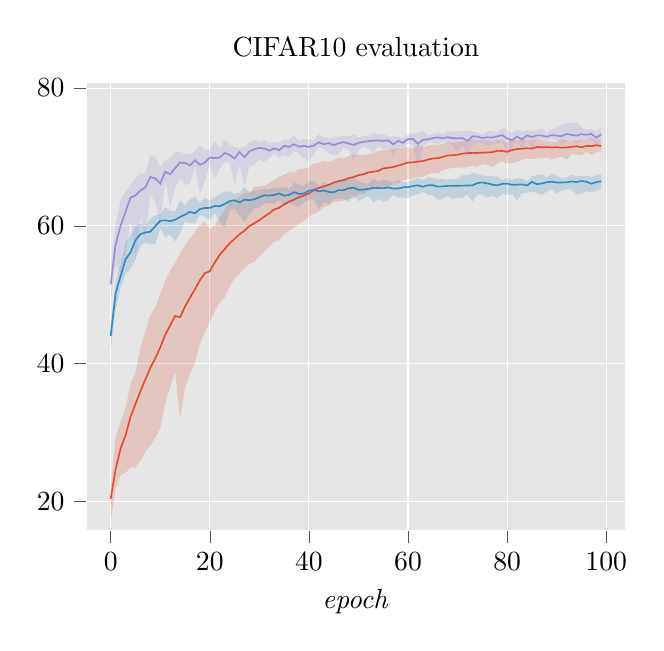
\begin{tikzpicture}

\definecolor{color0}{rgb}{0.886274509803922,0.290196078431373,0.2}
\definecolor{color1}{rgb}{0.203921568627451,0.541176470588235,0.741176470588235}
\definecolor{color2}{rgb}{0.596078431372549,0.556862745098039,0.835294117647059}

\begin{axis}[
axis background/.style={fill=white!89.8039215686275!black},
axis line style={white},
legend cell align={left},
legend style={fill opacity=0.8, draw opacity=1, text opacity=1, at={(0.97,0.03)}, anchor=south east, draw=white!80!black, fill=white!89.8039215686275!black},
log basis y={10},
tick align=outside,
tick pos=left,
title={CIFAR10 evaluation},
x grid style={white},
xlabel={\textit{epoch}},
xmajorgrids,
xmin=-4.95, xmax=103.95,
xtick style={color=white!33.3333333333333!black},
y grid style={white},
ymajorgrids,
ymin=15.7517645561491, ymax=80.8079673084566,
%ymode=log,
ytick style={color=white!33.3333333333333!black}
]
\path [fill=color0, fill opacity=0.2, very thin]
(axis cs:0,22.2756)
--(axis cs:0,16.9671)
--(axis cs:1,22.0553)
--(axis cs:2,23.8281)
--(axis cs:3,24.1787)
--(axis cs:4,24.9499)
--(axis cs:5,24.97)
--(axis cs:6,25.9115)
--(axis cs:7,27.2336)
--(axis cs:8,28.145)
--(axis cs:9,29.2167)
--(axis cs:10,30.6791)
--(axis cs:11,34.2949)
--(axis cs:12,36.5986)
--(axis cs:13,38.8321)
--(axis cs:14,32.0112)
--(axis cs:15,36.5785)
--(axis cs:16,38.5116)
--(axis cs:17,40.1042)
--(axis cs:18,42.8786)
--(axis cs:19,44.5413)
--(axis cs:20,46.1038)
--(axis cs:21,47.5561)
--(axis cs:22,48.9383)
--(axis cs:23,49.5893)
--(axis cs:24,51.1619)
--(axis cs:25,52.3638)
--(axis cs:26,52.9748)
--(axis cs:27,53.9463)
--(axis cs:28,54.4872)
--(axis cs:29,54.8177)
--(axis cs:30,55.599)
--(axis cs:31,56.3001)
--(axis cs:32,57.0112)
--(axis cs:33,57.7524)
--(axis cs:34,57.8826)
--(axis cs:35,58.7841)
--(axis cs:36,59.3049)
--(axis cs:37,59.7456)
--(axis cs:38,60.2965)
--(axis cs:39,60.7272)
--(axis cs:40,61.4183)
--(axis cs:41,61.7388)
--(axis cs:42,62.1294)
--(axis cs:43,62.6703)
--(axis cs:44,62.9307)
--(axis cs:45,63.4115)
--(axis cs:46,63.5517)
--(axis cs:47,63.6318)
--(axis cs:48,63.9223)
--(axis cs:49,64.0325)
--(axis cs:50,64.6735)
--(axis cs:51,64.5633)
--(axis cs:52,65.1542)
--(axis cs:53,65.2244)
--(axis cs:54,65.5349)
--(axis cs:55,65.5749)
--(axis cs:56,65.5449)
--(axis cs:57,66.1258)
--(axis cs:58,66.2059)
--(axis cs:59,66.5966)
--(axis cs:60,66.7368)
--(axis cs:61,66.897)
--(axis cs:62,67.0673)
--(axis cs:63,67.0873)
--(axis cs:64,67.528)
--(axis cs:65,67.6683)
--(axis cs:66,67.5982)
--(axis cs:67,68.109)
--(axis cs:68,68.2993)
--(axis cs:69,68.3994)
--(axis cs:70,68.4595)
--(axis cs:71,68.4395)
--(axis cs:72,68.5196)
--(axis cs:73,68.77)
--(axis cs:74,68.5296)
--(axis cs:75,68.9603)
--(axis cs:76,68.9002)
--(axis cs:77,68.5397)
--(axis cs:78,69.0605)
--(axis cs:79,69.4111)
--(axis cs:80,69.0204)
--(axis cs:81,69.1506)
--(axis cs:82,69.2608)
--(axis cs:83,69.6014)
--(axis cs:84,69.7917)
--(axis cs:85,69.6715)
--(axis cs:86,69.7917)
--(axis cs:87,69.8017)
--(axis cs:88,69.9119)
--(axis cs:89,69.6314)
--(axis cs:90,69.8718)
--(axis cs:91,70.0621)
--(axis cs:92,69.6014)
--(axis cs:93,70.4527)
--(axis cs:94,70.3325)
--(axis cs:95,70.2724)
--(axis cs:96,70.7532)
--(axis cs:97,70.3025)
--(axis cs:98,70.7031)
--(axis cs:99,70.8734)
--(axis cs:99,72.3958)
--(axis cs:99,72.3958)
--(axis cs:98,72.486)
--(axis cs:97,72.7764)
--(axis cs:96,72.4459)
--(axis cs:95,72.496)
--(axis cs:94,72.3357)
--(axis cs:93,72.2756)
--(axis cs:92,72.4159)
--(axis cs:91,72.5561)
--(axis cs:90,72.2055)
--(axis cs:89,72.2556)
--(axis cs:88,72.3458)
--(axis cs:87,72.4159)
--(axis cs:86,72.6763)
--(axis cs:85,72.496)
--(axis cs:84,72.4058)
--(axis cs:83,72.6262)
--(axis cs:82,72.3658)
--(axis cs:81,72.526)
--(axis cs:80,72.0753)
--(axis cs:79,72.4459)
--(axis cs:78,72.4559)
--(axis cs:77,72.2756)
--(axis cs:76,72.506)
--(axis cs:75,72.4559)
--(axis cs:74,72.4659)
--(axis cs:73,72.526)
--(axis cs:72,72.3658)
--(axis cs:71,72.2756)
--(axis cs:70,72.2155)
--(axis cs:69,72.0252)
--(axis cs:68,72.2456)
--(axis cs:67,71.845)
--(axis cs:66,71.7949)
--(axis cs:65,71.8049)
--(axis cs:64,71.6346)
--(axis cs:63,71.3842)
--(axis cs:62,71.7748)
--(axis cs:61,71.1739)
--(axis cs:60,71.5044)
--(axis cs:59,71.254)
--(axis cs:58,71.274)
--(axis cs:57,71.0938)
--(axis cs:56,71.0537)
--(axis cs:55,70.9635)
--(axis cs:54,70.9135)
--(axis cs:53,70.5028)
--(axis cs:52,70.4327)
--(axis cs:51,70.2524)
--(axis cs:50,70.3025)
--(axis cs:49,70.3926)
--(axis cs:48,70.1522)
--(axis cs:47,69.7516)
--(axis cs:46,69.9219)
--(axis cs:45,69.5513)
--(axis cs:44,69.3009)
--(axis cs:43,69.391)
--(axis cs:42,69.1907)
--(axis cs:41,69.0605)
--(axis cs:40,68.4195)
--(axis cs:39,68.3093)
--(axis cs:38,68.2492)
--(axis cs:37,67.6683)
--(axis cs:36,67.8486)
--(axis cs:35,67.4279)
--(axis cs:34,67.1474)
--(axis cs:33,66.6767)
--(axis cs:32,66.2159)
--(axis cs:31,65.8353)
--(axis cs:30,65.6951)
--(axis cs:29,65.7452)
--(axis cs:28,64.6935)
--(axis cs:27,64.8337)
--(axis cs:26,64.2628)
--(axis cs:25,63.6218)
--(axis cs:24,63.4816)
--(axis cs:23,62.3998)
--(axis cs:22,61.1378)
--(axis cs:21,60.1162)
--(axis cs:20,59.5753)
--(axis cs:19,60.607)
--(axis cs:18,60.1062)
--(axis cs:17,59.1046)
--(axis cs:16,58.2031)
--(axis cs:15,57.1915)
--(axis cs:14,55.9996)
--(axis cs:13,54.6474)
--(axis cs:12,53.5357)
--(axis cs:11,52.0333)
--(axis cs:10,50.1102)
--(axis cs:9,48.2071)
--(axis cs:8,47.0954)
--(axis cs:7,44.7416)
--(axis cs:6,42.2476)
--(axis cs:5,38.6819)
--(axis cs:4,37.0593)
--(axis cs:3,33.5737)
--(axis cs:2,31.5405)
--(axis cs:1,29.3269)
--(axis cs:0,22.2756)
--cycle;

\path [fill=color1, fill opacity=0.2, very thin]
(axis cs:0,45.7278)
--(axis cs:0,41.9205)
--(axis cs:1,47.765)
--(axis cs:2,51.0384)
--(axis cs:3,53.1349)
--(axis cs:4,53.6689)
--(axis cs:5,55.1028)
--(axis cs:6,57.051)
--(axis cs:7,57.6048)
--(axis cs:8,57.2884)
--(axis cs:9,57.3675)
--(axis cs:10,59.6519)
--(axis cs:11,58.3366)
--(axis cs:12,58.6926)
--(axis cs:13,57.7136)
--(axis cs:14,58.9498)
--(axis cs:15,60.6309)
--(axis cs:16,60.4331)
--(axis cs:17,60.3441)
--(axis cs:18,61.6297)
--(axis cs:19,61.3133)
--(axis cs:20,60.8386)
--(axis cs:21,61.9363)
--(axis cs:22,60.621)
--(axis cs:23,59.7805)
--(axis cs:24,62.2231)
--(axis cs:25,62.5198)
--(axis cs:26,61.5605)
--(axis cs:27,60.5815)
--(axis cs:28,61.6891)
--(axis cs:29,62.5791)
--(axis cs:30,62.5791)
--(axis cs:31,63.2812)
--(axis cs:32,63.301)
--(axis cs:33,63.1527)
--(axis cs:34,63.7757)
--(axis cs:35,62.8659)
--(axis cs:36,63.2615)
--(axis cs:37,63.0637)
--(axis cs:38,62.6385)
--(axis cs:39,63.4691)
--(axis cs:40,63.8153)
--(axis cs:41,63.8746)
--(axis cs:42,62.4308)
--(axis cs:43,63.4691)
--(axis cs:44,63.1428)
--(axis cs:45,63.8845)
--(axis cs:46,63.8647)
--(axis cs:47,63.8647)
--(axis cs:48,63.4395)
--(axis cs:49,64.468)
--(axis cs:50,63.5977)
--(axis cs:51,63.9735)
--(axis cs:52,64.3295)
--(axis cs:53,63.3604)
--(axis cs:54,63.924)
--(axis cs:55,63.5087)
--(axis cs:56,63.7065)
--(axis cs:57,64.4877)
--(axis cs:58,64.1021)
--(axis cs:59,64.1515)
--(axis cs:60,63.9735)
--(axis cs:61,64.4284)
--(axis cs:62,64.5372)
--(axis cs:63,64.9723)
--(axis cs:64,64.4877)
--(axis cs:65,64.4185)
--(axis cs:66,63.8153)
--(axis cs:67,63.8845)
--(axis cs:68,64.3691)
--(axis cs:69,63.8647)
--(axis cs:70,64.0922)
--(axis cs:71,64.0427)
--(axis cs:72,64.557)
--(axis cs:73,63.5186)
--(axis cs:74,64.6064)
--(axis cs:75,64.5668)
--(axis cs:76,64.1218)
--(axis cs:77,64.3888)
--(axis cs:78,63.9537)
--(axis cs:79,64.6756)
--(axis cs:80,64.5174)
--(axis cs:81,64.5767)
--(axis cs:82,63.6966)
--(axis cs:83,64.6855)
--(axis cs:84,64.824)
--(axis cs:85,64.9822)
--(axis cs:86,64.7251)
--(axis cs:87,64.4779)
--(axis cs:88,64.9921)
--(axis cs:89,65.269)
--(axis cs:90,64.6954)
--(axis cs:91,65.091)
--(axis cs:92,65.3283)
--(axis cs:93,65.2591)
--(axis cs:94,64.5273)
--(axis cs:95,64.6657)
--(axis cs:96,65.002)
--(axis cs:97,64.8833)
--(axis cs:98,65.1108)
--(axis cs:99,65.2888)
--(axis cs:99,67.5336)
--(axis cs:99,67.5336)
--(axis cs:98,67.3358)
--(axis cs:97,67.0985)
--(axis cs:96,67.2567)
--(axis cs:95,67.2271)
--(axis cs:94,67.2666)
--(axis cs:93,67.3952)
--(axis cs:92,67.0392)
--(axis cs:91,66.9699)
--(axis cs:90,67.3062)
--(axis cs:89,67.5831)
--(axis cs:88,67.0293)
--(axis cs:87,67.4941)
--(axis cs:86,67.3457)
--(axis cs:85,67.2073)
--(axis cs:84,66.4854)
--(axis cs:83,66.8809)
--(axis cs:82,66.9304)
--(axis cs:81,66.6733)
--(axis cs:80,66.9106)
--(axis cs:79,66.7029)
--(axis cs:78,67.1084)
--(axis cs:77,67.2271)
--(axis cs:76,67.1974)
--(axis cs:75,67.3161)
--(axis cs:74,67.5732)
--(axis cs:73,67.6523)
--(axis cs:72,67.3358)
--(axis cs:71,67.3952)
--(axis cs:70,66.7524)
--(axis cs:69,66.8315)
--(axis cs:68,66.6832)
--(axis cs:67,66.8315)
--(axis cs:66,66.8414)
--(axis cs:65,66.9403)
--(axis cs:64,67.049)
--(axis cs:63,66.6535)
--(axis cs:62,66.9502)
--(axis cs:61,66.6832)
--(axis cs:60,66.3667)
--(axis cs:59,66.337)
--(axis cs:58,66.6832)
--(axis cs:57,66.2678)
--(axis cs:56,66.5546)
--(axis cs:55,66.6832)
--(axis cs:54,66.3766)
--(axis cs:53,66.8315)
--(axis cs:52,66.1096)
--(axis cs:51,66.2282)
--(axis cs:50,66.4557)
--(axis cs:49,67.0985)
--(axis cs:48,66.7326)
--(axis cs:47,66.6337)
--(axis cs:46,66.4755)
--(axis cs:45,66.0502)
--(axis cs:44,66.0206)
--(axis cs:43,66.3172)
--(axis cs:42,65.7832)
--(axis cs:41,66.4854)
--(axis cs:40,66.426)
--(axis cs:39,65.9019)
--(axis cs:38,66.0502)
--(axis cs:37,66.2381)
--(axis cs:36,65.4173)
--(axis cs:35,65.625)
--(axis cs:34,65.4371)
--(axis cs:33,65.625)
--(axis cs:32,65.3184)
--(axis cs:31,65.3778)
--(axis cs:30,65.1899)
--(axis cs:29,65.1305)
--(axis cs:28,64.8932)
--(axis cs:27,65.625)
--(axis cs:26,64.8042)
--(axis cs:25,64.6262)
--(axis cs:24,65.0218)
--(axis cs:23,64.9624)
--(axis cs:22,64.5866)
--(axis cs:21,64.1416)
--(axis cs:20,63.6669)
--(axis cs:19,64.0328)
--(axis cs:18,63.3703)
--(axis cs:17,64.2801)
--(axis cs:16,63.8449)
--(axis cs:15,62.9747)
--(axis cs:14,63.7362)
--(axis cs:13,62.0945)
--(axis cs:12,62.1934)
--(axis cs:11,62.7176)
--(axis cs:10,61.6693)
--(axis cs:9,61.5012)
--(axis cs:8,61.1254)
--(axis cs:7,59.8794)
--(axis cs:6,60.3639)
--(axis cs:5,59.9288)
--(axis cs:4,58.6432)
--(axis cs:3,57.6543)
--(axis cs:2,54.3809)
--(axis cs:1,52.0372)
--(axis cs:0,45.7278)
--cycle;

\path [fill=color2, fill opacity=0.2, very thin]
(axis cs:0,54.153481)
--(axis cs:0,49.129747)
--(axis cs:1,54.252373)
--(axis cs:2,53.065665)
--(axis cs:3,55.676424)
--(axis cs:4,61.115506)
--(axis cs:5,54.924842)
--(axis cs:6,61.382516)
--(axis cs:7,58.356408)
--(axis cs:8,64.576741)
--(axis cs:9,63.399921)
--(axis cs:10,60.116693)
--(axis cs:11,66.742484)
--(axis cs:12,62.717563)
--(axis cs:13,65.516218)
--(axis cs:14,66.900712)
--(axis cs:15,65.921677)
--(axis cs:16,66.129351)
--(axis cs:17,68.571994)
--(axis cs:18,64.566851)
--(axis cs:19,66.574367)
--(axis cs:20,68.819225)
--(axis cs:21,66.821598)
--(axis cs:22,68.255538)
--(axis cs:23,69.323576)
--(axis cs:24,69.195016)
--(axis cs:25,66.040348)
--(axis cs:26,68.918117)
--(axis cs:27,65.704114)
--(axis cs:28,68.710443)
--(axis cs:29,68.87856)
--(axis cs:30,69.649921)
--(axis cs:31,69.293908)
--(axis cs:32,69.768592)
--(axis cs:33,70.549842)
--(axis cs:34,69.877373)
--(axis cs:35,70.213608)
--(axis cs:36,70.015823)
--(axis cs:37,70.826741)
--(axis cs:38,70.480617)
--(axis cs:39,69.768592)
--(axis cs:40,69.412579)
--(axis cs:41,70.44106)
--(axis cs:42,71.400316)
--(axis cs:43,71.143196)
--(axis cs:44,70.460839)
--(axis cs:45,70.223497)
--(axis cs:46,70.352057)
--(axis cs:47,71.370649)
--(axis cs:48,70.994858)
--(axis cs:49,69.541139)
--(axis cs:50,70.866297)
--(axis cs:51,71.538766)
--(axis cs:52,71.212421)
--(axis cs:53,70.530063)
--(axis cs:54,71.696994)
--(axis cs:55,71.064082)
--(axis cs:56,71.192642)
--(axis cs:57,70.094937)
--(axis cs:58,71.380538)
--(axis cs:59,71.301424)
--(axis cs:60,71.934335)
--(axis cs:61,71.657437)
--(axis cs:62,68.453323)
--(axis cs:63,71.420095)
--(axis cs:64,72.082674)
--(axis cs:65,72.072785)
--(axis cs:66,71.914557)
--(axis cs:67,72.221123)
--(axis cs:68,72.349684)
--(axis cs:69,71.568434)
--(axis cs:70,70.658623)
--(axis cs:71,71.74644)
--(axis cs:72,70.154272)
--(axis cs:73,71.716772)
--(axis cs:74,71.954114)
--(axis cs:75,72.013449)
--(axis cs:76,71.677215)
--(axis cs:77,71.894778)
--(axis cs:78,71.973892)
--(axis cs:79,72.359573)
--(axis cs:80,70.035601)
--(axis cs:81,71.400316)
--(axis cs:82,72.102453)
--(axis cs:83,71.123418)
--(axis cs:84,72.39913)
--(axis cs:85,70.935522)
--(axis cs:86,72.676028)
--(axis cs:87,72.606804)
--(axis cs:88,72.478244)
--(axis cs:89,72.626582)
--(axis cs:90,72.478244)
--(axis cs:91,71.677215)
--(axis cs:92,72.290348)
--(axis cs:93,72.300237)
--(axis cs:94,72.082674)
--(axis cs:95,72.27057)
--(axis cs:96,72.409019)
--(axis cs:97,72.458465)
--(axis cs:98,71.706883)
--(axis cs:99,72.26068)
--(axis cs:99,74.278085)
--(axis cs:99,74.278085)
--(axis cs:98,73.684731)
--(axis cs:97,74.060522)
--(axis cs:96,73.83307)
--(axis cs:95,74.386867)
--(axis cs:94,75.019778)
--(axis cs:93,74.920886)
--(axis cs:92,74.950554)
--(axis cs:91,74.673655)
--(axis cs:90,74.258307)
--(axis cs:89,73.951741)
--(axis cs:88,73.486946)
--(axis cs:87,74.149525)
--(axis cs:86,73.862737)
--(axis cs:85,73.753956)
--(axis cs:84,73.882516)
--(axis cs:83,73.714399)
--(axis cs:82,73.981408)
--(axis cs:81,73.397943)
--(axis cs:80,74.109968)
--(axis cs:79,74.179193)
--(axis cs:78,73.506725)
--(axis cs:77,73.82318)
--(axis cs:76,73.724288)
--(axis cs:75,73.239715)
--(axis cs:74,73.516614)
--(axis cs:73,73.704509)
--(axis cs:72,73.813291)
--(axis cs:71,73.664953)
--(axis cs:70,73.842959)
--(axis cs:69,73.585839)
--(axis cs:68,73.773734)
--(axis cs:67,73.289161)
--(axis cs:66,73.575949)
--(axis cs:65,73.358386)
--(axis cs:64,73.160601)
--(axis cs:63,73.813291)
--(axis cs:62,73.575949)
--(axis cs:61,73.407832)
--(axis cs:60,73.299051)
--(axis cs:59,72.735364)
--(axis cs:58,72.91337)
--(axis cs:57,73.002373)
--(axis cs:56,72.933149)
--(axis cs:55,73.378165)
--(axis cs:54,73.338608)
--(axis cs:53,73.486946)
--(axis cs:52,73.150712)
--(axis cs:51,73.022152)
--(axis cs:50,72.844146)
--(axis cs:49,73.318829)
--(axis cs:48,72.982595)
--(axis cs:47,73.022152)
--(axis cs:46,72.883703)
--(axis cs:45,72.824367)
--(axis cs:44,72.685918)
--(axis cs:43,72.844146)
--(axis cs:42,73.338608)
--(axis cs:41,72.349684)
--(axis cs:40,72.616693)
--(axis cs:39,72.626582)
--(axis cs:38,72.369462)
--(axis cs:37,73.239715)
--(axis cs:36,72.52769)
--(axis cs:35,72.547468)
--(axis cs:34,72.033228)
--(axis cs:33,72.161788)
--(axis cs:32,71.924446)
--(axis cs:31,72.478244)
--(axis cs:30,72.201345)
--(axis cs:29,72.488133)
--(axis cs:28,72.142009)
--(axis cs:27,71.420095)
--(axis cs:26,71.311313)
--(axis cs:25,71.439873)
--(axis cs:24,71.795886)
--(axis cs:23,72.52769)
--(axis cs:22,71.281646)
--(axis cs:21,72.409019)
--(axis cs:20,71.044304)
--(axis cs:19,71.034415)
--(axis cs:18,71.687104)
--(axis cs:17,70.866297)
--(axis cs:16,70.450949)
--(axis cs:15,70.381725)
--(axis cs:14,70.727848)
--(axis cs:13,70.747627)
--(axis cs:12,69.857595)
--(axis cs:11,69.551028)
--(axis cs:10,68.502769)
--(axis cs:9,69.946598)
--(axis cs:8,70.352057)
--(axis cs:7,67.592959)
--(axis cs:6,67.622627)
--(axis cs:5,66.960047)
--(axis cs:4,65.990902)
--(axis cs:3,64.893196)
--(axis cs:2,63.815269)
--(axis cs:1,60.215585)
--(axis cs:0,54.153481)
--cycle;

\addplot [semithick, color0]
table {%
0 20.3896198272705
1 24.7235527038574
2 27.6973209381104
3 29.6133804321289
4 32.2686347961426
5 34.1556663513184
6 35.9986000061035
7 37.7153549194336
8 39.4130516052246
9 40.8022880554199
10 42.3437614440918
11 44.1957244873047
13 46.9310646057129
14 46.7427825927734
15 48.2922515869141
16 49.5753059387207
17 50.7982864379883
18 52.1123924255371
19 53.132022857666
20 53.4134674072266
21 54.6864967346191
22 55.8002662658691
24 57.4719657897949
26 58.7840576171875
27 59.3119049072266
28 59.9799652099609
30 60.8153076171875
31 61.360179901123
32 61.8129081726074
33 62.3918151855469
34 62.6311988830566
35 63.1410140991211
36 63.5236396789551
37 63.8120994567871
38 64.1576385498047
40 64.6895217895508
41 65.2303619384766
42 65.5038070678711
44 65.9635467529297
45 66.2730560302734
46 66.4983901977539
47 66.6316070556641
48 66.9350814819336
49 67.0803298950195
50 67.3437423706055
51 67.485969543457
52 67.7634201049805
53 67.8525772094727
54 67.9847717285156
55 68.3333206176758
57 68.5366668701172
60 69.184700012207
61 69.2127532958984
62 69.340934753418
63 69.3960418701172
64 69.6223831176758
65 69.7736358642578
66 69.8207244873047
68 70.2133483886719
69 70.2533874511719
70 70.3355331420898
71 70.4787521362305
72 70.5578842163086
73 70.5919418334961
74 70.5839157104492
77 70.6930999755859
78 70.8844375610352
79 70.8724136352539
80 70.7562103271484
81 71.0045700073242
82 71.1488418579102
84 71.265022277832
85 71.2139434814453
86 71.4463119506836
87 71.3992462158203
88 71.4373092651367
89 71.3601760864258
90 71.421272277832
91 71.3481521606445
92 71.377197265625
94 71.5594787597656
95 71.4132537841797
96 71.5885391235352
97 71.5755310058594
98 71.6977233886719
99 71.6085662841797
};
%\addlegendentry{cudnn}
\addplot [semithick, color1]
table {%
0 44.0516204833984
1 50.2492065429688
2 52.7126274108887
3 55.1443901062012
4 56.1491165161133
5 57.9034729003906
6 58.8113021850586
7 59.0387763977051
8 59.1574554443359
10 60.7456359863281
11 60.8089485168457
12 60.6892547607422
13 60.8831024169922
14 61.2964782714844
15 61.6297492980957
16 62.0361862182617
17 61.8235778808594
18 62.4376792907715
19 62.5979080200195
20 62.6107597351074
21 62.8916244506836
22 62.8382186889648
23 63.1714935302734
24 63.6026573181152
25 63.7124252319336
26 63.4157447814941
27 63.7885627746582
28 63.7302131652832
29 63.8558158874512
31 64.4442367553711
32 64.3858871459961
33 64.4986190795898
34 64.7023239135742
35 64.384880065918
36 64.4887237548828
37 64.8882522583008
38 64.6390609741211
39 64.7013626098633
40 65.1067886352539
41 65.1928405761719
42 65.018798828125
43 65.1433868408203
44 64.9199142456055
45 64.8565979003906
46 65.1968154907227
47 65.1730575561523
48 65.4549026489258
49 65.5369873046875
50 65.2264404296875
51 65.2600936889648
52 65.3639450073242
53 65.5271148681641
55 65.4687576293945
56 65.5656661987305
57 65.4153289794922
58 65.4272003173828
59 65.5943450927734
60 65.6220397949219
61 65.7792816162109
62 65.8831100463867
63 65.6873016357422
64 65.8919906616211
65 65.8989410400391
66 65.6912460327148
68 65.7990570068359
71 65.8386001586914
73 65.8851013183594
74 66.2143783569336
75 66.2994537353516
76 66.1688995361328
77 65.97705078125
78 65.8939971923828
79 66.0967102050781
80 66.1382675170898
81 65.9612274169922
82 65.9701385498047
83 66.0255126953125
84 65.8593902587891
85 66.385498046875
86 66.0532150268555
87 66.1550827026367
88 66.3340606689453
89 66.4082260131836
90 66.2965087890625
92 66.3123016357422
93 66.4428482055664
94 66.3647308349609
95 66.503173828125
96 66.3993301391602
97 66.1224365234375
98 66.3479156494141
99 66.4685516357422
};
%\addlegendentry{libtorch}
\addplot [semithick, color2]
table {%
0 51.5002021789551
1 57.3081474304199
2 60.0267066955566
3 62.0520248413086
4 64.1020660400391
5 64.394775390625
6 65.1335144042969
7 65.5992965698242
8 67.0895919799805
9 66.8858795166016
10 66.1303329467773
11 67.8550338745117
12 67.4782485961914
13 68.3860855102539
14 69.1880950927734
15 69.1406173706055
16 68.7737350463867
17 69.5174102783203
18 68.8686599731445
19 69.1821517944336
20 69.9248504638672
21 69.8308868408203
22 69.911994934082
23 70.5824661254883
24 70.2966766357422
25 69.7725448608398
26 70.7248916625977
27 69.9554901123047
28 70.8316879272461
29 71.1194610595703
30 71.3281173706055
31 71.2282333374023
32 70.9206924438477
33 71.2470245361328
34 70.9968338012695
35 71.6040267944336
36 71.4784469604492
37 71.8482971191406
38 71.5002059936523
39 71.6139297485352
40 71.4586715698242
41 71.6663360595703
42 72.128173828125
43 71.856201171875
44 72.0124664306641
45 71.7306137084961
46 71.9887313842773
47 72.1588287353516
49 71.7464447021484
50 72.0470657348633
51 72.2023391723633
53 72.372428894043
54 72.3951721191406
55 72.3160705566406
56 72.4129638671875
57 71.8334655761719
58 72.3318939208984
59 72.0440979003906
60 72.5929489135742
61 72.6176834106445
62 71.9155349731445
63 72.4723205566406
64 72.5632858276367
65 72.7452621459961
66 72.842170715332
67 72.7225036621094
68 72.861946105957
69 72.724479675293
70 72.6987762451172
71 72.7412872314453
72 72.3299026489258
73 72.9895172119141
74 72.9469985961914
75 72.7403106689453
76 72.8609466552734
77 72.8125076293945
79 73.1843414306641
80 72.6790008544922
81 72.4228591918945
82 72.9578704833984
83 72.5573501586914
84 73.1269683837891
85 72.8965606689453
86 73.1388549804688
87 73.125
88 72.9410705566406
89 73.1714859008789
91 73.0221633911133
92 73.3247680664062
94 73.0973052978516
95 73.3119125366211
96 73.203125
97 73.3445358276367
98 72.7877655029297
99 73.2852096557617
};
%\addlegendentry{pytorch}
\end{axis}

\end{tikzpicture}

        \end{adjustbox}
    \end{subfigure}
    \caption{Comparison of accuracy for PyTorch, LibTorch, and cuDNN implementations during training and evaluation. Solid line corresponds to mean while shaded regions correspond to min and max. Time is measured in units of \textit{epoch} $\times$ \textit{average epoch time}. }
    \label{fig:accuracy_results}
\end{figure*}
